% CPSC 4900 Senior Project
% A Conservative Post-Segmentation Pipeline for Large-Scale Connectomics
% Yale University, Spring 2026

\documentclass[12pt,twoside]{report}
\usepackage[utf8]{inputenc}
\usepackage{times}
\usepackage{graphicx}
\usepackage{amsmath}
\usepackage{amssymb}
\graphicspath{ {images/} }
\usepackage{caption}
\usepackage{subcaption}
\usepackage[a4paper,width=150mm,top=35mm,bottom=35mm,bindingoffset=6mm]{geometry}

\usepackage{float}
\usepackage{url}
\urlstyle{same}
\usepackage[%
  colorlinks,bookmarksopen,bookmarksnumbered,citecolor=black,urlcolor=black,linkcolor=black
]{hyperref}

\usepackage{tikz}
\usetikzlibrary{shapes.geometric, arrows.meta, positioning}
\usepackage{titlesec}
\usepackage{booktabs}
\usepackage{tabularx}
\usepackage{ragged2e}
\usepackage{xcolor}

% Customize chapter title format
\titleformat{\chapter}[hang]
  {\normalfont\huge\bfseries}{\thechapter}{1em}{}
\titlespacing*{\chapter}{0pt}{35pt}{20pt}

\bibliographystyle{plainnat}
\usepackage[sorting=none]{biblatex}
\addbibresource{references.bib}
\hypersetup{linkcolor=black}

% Float layout: prevent figures from overflowing into footer/page numbers.
% A float occupying more than 85% of a text page goes to a dedicated float page.
% At least 15% of a text page must be text before a bottom float is placed.
\renewcommand{\floatpagefraction}{0.85}
\renewcommand{\textfraction}{0.10}
\renewcommand{\topfraction}{0.90}
\renewcommand{\bottomfraction}{0.75}
\setlength{\floatsep}{12pt plus 2pt minus 2pt}
\setlength{\textfloatsep}{16pt plus 2pt minus 4pt}
\setlength{\intextsep}{12pt plus 2pt minus 2pt}

\begin{document}

\begin{titlepage}
\centering
\vspace*{2cm}

{\Huge\bfseries A Conservative Post-Segmentation Pipeline\\[0.4em]
for Large-Scale Connectomics:\\[0.4em]
Graph-Based Neural Split Detection\\[0.4em]
in Volumetric EM and XNH Data\par}

\vspace{2.5cm}

{\LARGE [YOUR NAME]\par}

\vspace{1.5cm}

{\large CPSC 4900 --- Senior Project\\
Department of Computer Science\\
Yale University\par}

\vspace{1.2cm}

{\large Advisor: Dr. Aaron T. Kuan\\
Kuan Lab, Yale School of Medicine\par}

\vspace{1.2cm}

{\large Spring 2026\par}

\vfill

{\small
Submitted in partial fulfillment of the requirements\\
for the Bachelor of Science in Computer Science\\
Yale University
}

\end{titlepage}


\chapter*{Acknowledgements}
\addcontentsline{toc}{chapter}{Acknowledgements}

I would like to express my sincere gratitude to my advisors, Dr.\ Xiuye Chen
(Yale Department of Computer Science) and Dr.\ Aaron T.\ Kuan (Kuan Lab, Yale
School of Medicine). Dr.\ Chen provided invaluable guidance on computer science
methodology, software design, and academic communication throughout the project.
Dr.\ Kuan and the Kuan Lab provided the domain expertise, connectomics datasets,
and neuroscience mentorship that shaped the direction and evaluation of this work.

The XPRESS challenge data used in this work was provided through the challenge
infrastructure maintained by the challenge organizers. The CREMI benchmark data
is publicly available through the CREMI challenge. Thanks also to the Yale
Department of Computer Science for the resources and academic environment that
supported this work. This project was completed as part of the CPSC 4900 Senior
Project requirement.

{
  \hypersetup{linkcolor=black}
  \tableofcontents
}

\clearpage

\chapter*{Abstract}
\addcontentsline{toc}{chapter}{Abstract}

Large-scale connectomics --- the mapping of neural circuits from volumetric
electron microscopy (EM) and X-ray nano-holotomography (XNH) data --- requires
automated segmentation of three-dimensional image volumes into individual neuronal
fragments. State-of-the-art automated segmenters produce fragments with high accuracy
but inevitably introduce \emph{split errors}, where a single neuron is represented as
multiple disconnected fragments. Correcting these errors at the scale of modern
connectomics datasets (tens to hundreds of teravoxels) demands automated
proofreading pipelines that can detect and propose corrections for split errors
with high recall and with explicit handling of uncertainty.

This report presents a modular, conservative post-segmentation pipeline that
takes the output of an automated segmenter and produces a graph-based
connectivity representation with confidence-annotated merge proposals. The pipeline
operates in six stages: fragment extraction with TEASAR skeletonization, graph
construction via a skeleton-node KD-tree index, candidate generation with a
four-factor composite scoring model, conservative three-outcome rule-based
validation (ACCEPT / REJECT / AMBIGUOUS), structure assembly, and multi-format
export. Critically, the pipeline treats uncertainty as a first-class output ---
ambiguous connections are preserved for human review rather than forced to a
binary decision.

Two key innovations drive the approach's effectiveness on axon-dominated datasets.
First, a \emph{skeleton-node graph} indexes every skeleton node from every fragment
(rather than only degree-1 endpoints), exposing interior splits along long axons
that an endpoint-only graph cannot detect. Second, \emph{distance-conditioned
scoring} switches from a proximity-weighted composite to a proximity-free,
alignment-continuity-weighted score for long-range candidate pairs, preventing
the artificial suppression of genuine long-range splits.

Evaluated on the CREMI Drosophila EM benchmark, the pipeline achieves
Precision = 1.000, Recall = 0.909, and F1 = 0.952. On the XPRESS mouse white
matter XNH challenge --- the primary domain-appropriate benchmark --- the pipeline
achieves Coverage = 83.5\% and Recall = 0.994 on the training volume (Experiment~17),
and Coverage = 72.4\%, Recall = 0.885 on the fully held-out validation volume
(Experiment~23), confirming that the learned thresholds generalize without
overfitting. The pipeline is validated by 428 automated tests and includes a
reproducible visual diagnostic report for per-candidate inspection.

The main open challenge is precision: approximately 354{,}000 false-positive
merge proposals are generated alongside 1{,}245 true positives at XPRESS scale
(Precision $\approx$ 0.004), reflecting the difficulty of discriminating
same-axon from different-axon long-range pairs in myelinated white matter using
geometric features alone. Future work targets this gap through improved scoring
and lightweight machine-learned filters.


\chapter{Introduction}
Understanding the brain at the level of individual synaptic connections requires
mapping the complete wiring diagram --- the \emph{connectome} --- of a neural
circuit. Modern connectomics workflows acquire volumetric image stacks of brain
tissue using electron microscopy (EM) or X-ray nano-holotomography (XNH), then
apply automated deep-learning segmenters to delineate individual neurons within
those volumes~\cite{januszewski2018high,lin2021pytorch}. This process has enabled
landmark reconstructions at increasingly large scales, culminating in full-cortex
and whole-brain datasets containing tens of thousands of neurons and hundreds of
millions of synapses~\cite{microns2025}.

Despite rapid progress in segmentation quality, automated segmenters remain
imperfect. They produce two types of errors: \emph{merge errors}, where
two distinct neurons are incorrectly fused into one segment, and \emph{split errors},
where a single neuron is fragmented into multiple disconnected pieces. Split
errors are particularly prevalent in elongated structures such as axons, where
slight imaging artifacts, staining variation, or object boundaries that are
difficult to resolve cause segmenters to break a continuous process into two or
more isolated fragments. At the scale of a full cortex reconstruction, a single
well-segmented volume may contain hundreds of thousands of split errors that must
be identified and corrected before the connectivity graph is reliable
enough for downstream neuroscience~\cite{plaza2018analyzing}.

Manual proofreading --- having human experts identify and repair segmentation
errors --- is the bottleneck in every large-scale connectomics project. A skilled
proofreader can correct perhaps a few hundred merge decisions per hour; a modern
dataset may require millions. Automated proofreading tools that propose high-recall
merge corrections, leaving only ambiguous cases for human review, are therefore
essential infrastructure for the field~\cite{dorkenwald2022cave}.

\section*{The Problem This Work Addresses}

This project targets \textbf{split detection and correction proposal} in
post-segmentation connectomics pipelines. Given a voxel-wise segmentation
volume (the output of an automated segmenter), the pipeline must:

\begin{enumerate}
  \item Identify all pairs of fragments that are likely pieces of the same neuron
        (\emph{split candidates}).
  \item Score and filter these pairs conservatively, accepting only those for which
        evidence strongly supports a merge.
  \item Explicitly flag uncertain pairs rather than forcing them to a binary decision.
  \item Produce outputs in formats consumable by downstream proofreading tools.
\end{enumerate}

The domain of primary interest is \textbf{myelinated axons in mouse white matter},
as captured by XNH imaging --- the XPRESS challenge dataset~\cite{xpress2023}.
Myelinated axons are predominantly tubular structures with consistent cross-sectional
geometry, making geometric alignment and curvature features informative proxies
for merge plausibility. This is in contrast to dendritic arbors, where branching
angles can be nearly orthogonal and geometric features are less discriminative.

\section*{Contributions}

The main contributions of this work are:

\begin{enumerate}
  \item \textbf{A complete, modular post-segmentation pipeline} implemented in
        Python, with YAML-configurable parameters, six processing stages, and
        multi-format export. The pipeline is fully open-source and validated by
        428 automated unit and integration tests.

  \item \textbf{The skeleton-node graph construction method}, which indexes every
        node from every TEASAR skeleton in a single KD-tree and queries the full
        node set for proximity-based edge creation. This exposes interior splits
        along long axons that an endpoint-only graph cannot represent, producing
        a 47-percentage-point improvement in oracle coverage on XPRESS (from 23\%
        to 79.8\% in a single change).

  \item \textbf{Distance-conditioned composite scoring}, which switches the
        candidate score weighting from a proximity-dominated formula to a
        proximity-free, alignment-continuity-weighted formula for long-range
        pairs (gap $> 1000$~nm). This prevents the suppression of genuine long-range
        splits whose proximity score decays to near zero despite strong directional
        alignment.

  \item \textbf{A three-outcome validation model} (ACCEPT / REJECT / AMBIGUOUS)
        with seven composable, configurable rules. The AMBIGUOUS outcome
        explicitly preserves uncertainty rather than forcing binary decisions,
        making the pipeline suitable for integration with human-in-the-loop
        proofreading workflows.

  \item \textbf{Quantitative evaluation on two benchmarks}: CREMI (F1 = 0.952,
        Precision = 1.000) and XPRESS (Recall = 0.994 on training, Recall = 0.885
        on a fully held-out validation volume), with 23 documented experiments
        tracing the development of each improvement.
\end{enumerate}

\section*{Report Organization}

Chapter~\ref{ch:background} provides background on connectomics imaging, automated
segmentation, and the XPRESS challenge. Chapter~\ref{ch:methodology} describes
the pipeline design and all algorithmic components in detail.
Chapter~\ref{ch:results} presents quantitative results across all experiments.
Chapter~\ref{ch:relatedwork} surveys related proofreading and graph-construction
approaches. Chapter~\ref{ch:conclusion} summarizes the main findings and
challenges, and Chapter~\ref{ch:futurework} outlines the plan for the remainder
of the semester.


\chapter{Background} \label{ch:background}
\section{Connectomics and Volumetric Imaging}

Connectomics is the study of neural wiring diagrams at synaptic resolution.
A connectome maps which neurons connect to which, with what synaptic strength,
and through which anatomical pathways. To obtain this information, researchers
section brain tissue into ultrathin slices (30--50~nm thick for EM; thicker
sections are used for XNH), image each slice, and reconstruct the
three-dimensional morphology of every neuron computationally.

Two imaging modalities are relevant to this work:

\paragraph{Electron Microscopy (EM).}
Serial-section transmission EM and focused ion beam scanning EM (FIB-SEM)
achieve 4--8~nm lateral resolution, sufficient to resolve individual synaptic
vesicles. The CREMI dataset~\cite{cremi2016} used in this work is a
$1250 \times 1250 \times 125$ voxel volume of \emph{Drosophila} larval brain
at $4 \times 4 \times 40$~nm resolution. The density of membranes and
organelles in EM images makes segmentation challenging: membranes appear as
bright thin sheets that segmenters must trace accurately.

\paragraph{X-ray Nano-Holotomography (XNH).}
XNH uses synchrotron X-rays to image brain tissue in three dimensions without
physical sectioning. It achieves lower resolution than EM (typically 25--33~nm
isotropic) but can image much larger volumes non-destructively. The XPRESS
challenge~\cite{xpress2023} uses a $699 \times 699 \times 699$ voxel volume of
mouse white matter at 33~nm isotropic resolution. Myelinated axons appear as
bright tubular structures surrounded by darker myelin sheaths, giving them
a characteristic ring-like cross-section that aids geometric reasoning.

\section{Automated Neural Segmentation}

Modern neural segmenters use deep convolutional networks, typically operating
on affinity predictions (per-voxel estimates of whether neighboring voxels
belong to the same object). Affinity maps are then processed by a watershed
or flood-filling algorithm to produce a label volume where each integer value
identifies a unique putative neuron fragment.

Flood-filling networks~\cite{januszewski2018high} are among the most accurate
segmenters: a convolutional network iteratively ``fills'' a segment from a seed,
deciding at each step whether to extend the current object or stop. Despite
high accuracy, all automated approaches produce residual errors.

\section{Segmentation Errors: Splits and Merges}

Segmentation errors fall into two categories:

\begin{description}
  \item[Merge errors] Two distinct neurons are assigned the same label. A merge
        introduces a false synapse (two neurons that appear connected when they
        are not) and is considered the more serious error type.
  \item[Split errors] A single neuron is broken into multiple fragments with
        distinct labels. Splits are more common than merges in long, thin structures
        like axons, where slight imaging artifacts or membrane contrast variation
        can interrupt a segmenter's flood-fill.
\end{description}

The XPRESS challenge reports that the baseline segmenter produces 1{,}499
ground-truth merge pairs across the training volume, with each pair representing
one split error that the pipeline must detect and propose to merge. The challenge
is to accept as many true pairs as possible (high recall) while rejecting
cross-axon false positives (high precision).

\section{Skeletonization}

Skeleton extraction converts a volumetric label into a compact graph of
centerline nodes and edges, capturing the topology of the neuron's morphology.
The TEASAR algorithm (Tree-structure Extraction Algorithm for Accurate and Robust
Skeletons)~\cite{sato2000teasar} traces a tree-structured skeleton by finding
shortest paths to a set of ``target'' voxels identified via distance-transform
analysis. TEASAR produces compact, well-centered skeletons with configurable
branch sensitivity. We use the \texttt{kimimaro}~\cite{kimimaro} Python
implementation, which supports GPU acceleration and multi-label batch processing.

Skeleton endpoints (degree-1 nodes in the skeleton graph) are natural
connection points: a true split typically produces two fragments whose free
endpoints point toward each other across the gap. However, for long axons that
are split in the interior (far from either end), the relevant skeleton nodes are
\emph{interior} nodes, not endpoints. This is a key observation that motivates the
skeleton-node graph construction described in Chapter~\ref{ch:methodology}.

\section{The XPRESS Challenge}

The XPRESS (X-ray nano-holotomography Processing for Evaluation of Segmentation
Software) challenge~\cite{xpress2023} provides:

\begin{itemize}
  \item A baseline segmentation volume (\texttt{baseline\_seg\_full.h5}): the
        output of an automated segmenter applied to mouse white matter XNH data.
        The volume is $699^3$ voxels at 33~nm isotropic resolution.
  \item A ground-truth skeleton dataset (\texttt{XPRESS\_training\_skels.npz}):
        manually traced skeleton graphs for the true axon trajectories, used as
        a proofreading oracle.
  \item A held-out validation volume (\texttt{baseline\_seg\_validation.h5}) with
        203 ground-truth merge pairs, used to evaluate generalization.
\end{itemize}

Ground-truth evaluation proceeds as follows: for each true axon trajectory, the
two baseline-segmentation fragments whose label IDs contain the most ground-truth
skeleton nodes at either end of the trajectory define an oracle merge pair. A
pipeline \emph{covers} a pair if it generates at least one candidate connecting
those two fragments. Of the covered pairs, those that are also accepted constitute
true positives.

\section{Prior Approaches to Automated Proofreading}

Early proofreading systems were purely manual, relying on human experts working
in tools such as CATMAID or Neuroglancer to trace axons and correct errors. The
scale of modern datasets has made fully manual proofreading infeasible, motivating
a shift toward human-in-the-loop systems~\cite{dorkenwald2022cave} where
algorithms propose corrections and humans verify only the uncertain cases.

Automated correction proposal systems generally follow one of two paradigms:
\emph{voxel-level} approaches, which re-run or fine-tune segmentation on regions
flagged as likely errors, and \emph{graph-level} approaches, which reason about
fragment-to-fragment merge plausibility using geometric or learned features.
This work falls in the latter category, operating entirely in the post-segmentation
graph domain without re-examining raw image data.


\chapter{Methodology} \label{ch:methodology}
\section{Design Philosophy}

The pipeline is structured as a graph-level proofreader: the input segmentation
volume is reduced to a set of fragment skeletons in the first stage, and every
subsequent decision (graph construction, candidate scoring, rule-based
validation, assembly) operates on skeleton geometry and fragment-level summary
statistics --- never on raw voxels. The voxel segmentation is the early input
and the late rendering target; the computational substrate for split detection
is the skeleton. This places the pipeline in the same tradition as NEURD
\cite{celii2025neurd}, Joyce et al.~\cite{joyce2023mesh}, and
ConnectomeBench~\cite{brown2025connectomebench}, which likewise reason over
mesh or skeleton representations rather than image patches.

Within this overall design, three principles govern the decision logic. First,
\textbf{conservative correctness}: a merge that should not happen is worse
than a merge proposal that is correctly rejected, so the pipeline never forces
an ambiguous decision; uncertainty is output explicitly as a third outcome
(AMBIGUOUS). Second, \textbf{modularity}: each stage can be run independently,
with intermediate results saved to disk and re-used across parameter sweeps.
Third, \textbf{reproducibility}: all parameters are controlled through a
single YAML configuration file, and random seeds are fixed, so the same
config always produces the same output.

The six-stage pipeline is shown in Figure~\ref{fig:pipeline}. The remainder
of this chapter describes each stage.

\begin{figure}[H]
\centering
\begin{tikzpicture}[
  node distance = 4.5mm,
  every node/.style  = {align=center},
  %--- node styles ---
  io/.style = {
    draw, ellipse,
    minimum width = 62mm, minimum height = 9mm,
    fill = gray!12, draw = gray!55, line width = 0.65pt,
    font = \small\bfseries,
  },
  stage/.style = {
    draw, rounded corners = 5pt,
    minimum width = 90mm,
    inner xsep = 10pt, inner ysep = 7pt,
    fill = blue!7, draw = blue!35!black, line width = 0.65pt,
  },
  key/.style = {stage, fill = orange!7, draw = orange!40!black},
  out/.style = {stage, fill = green!7, draw = green!45!black},
  %--- arrow style ---
  arr/.style = {
    -{Stealth[length=5pt, width=4pt]},
    line width = 0.9pt, color = gray!60!black,
  },
]

%% Input node
\node[io] (inp) {Segmentation Volume};

%% Stage 1
\node[stage, below=of inp] (s1) {
  {\small\bfseries [1]\enspace Fragment Extraction}\\[2pt]
  {\footnotesize\color{gray!55!black}
    Connected-component extraction $\cdot$ TEASAR skeletonisation $\cdot$ chunk stitching}
};

%% Stage 2
\node[stage, below=of s1] (s2) {
  {\small\bfseries [2]\enspace Graph Construction}\\[2pt]
  {\footnotesize\color{gray!55!black}
    Skeleton-node KD-tree $\cdot$ optional long-range endpoint pass}
};

%% Stage 3
\node[stage, below=of s2] (s3) {
  {\small\bfseries [3]\enspace Candidate Generation}\\[2pt]
  {\footnotesize\color{gray!55!black}
    Composite scoring $\cdot$ distance-conditioned weights}
};

%% Stage 4 — highlighted as the key decision stage
\node[key, below=of s3] (s4) {
  {\small\bfseries [4]\enspace Conservative Validation}\\[2pt]
  {\footnotesize\color{gray!55!black}
    7 configurable rules $\cdot$ three outcomes: \textbf{accept} / \textbf{reject} / \textbf{ambiguous}}
};

%% Stage 5
\node[stage, below=of s4] (s5) {
  {\small\bfseries [5]\enspace Assembly}\\[2pt]
  {\footnotesize\color{gray!55!black}
    Connected-component merging $\cdot$ cycle detection $\cdot$ topology checks}
};

%% Stage 6 — output
\node[out, below=of s5] (s6) {
  {\small\bfseries [6]\enspace Export}\\[2pt]
  {\footnotesize\color{gray!55!black}
    CSV $\cdot$ GraphML $\cdot$ SWC $\cdot$ Neuroglancer annotations}
};

%% Arrows
\draw[arr] (inp) -- (s1);
\draw[arr] (s1)  -- (s2);
\draw[arr] (s2)  -- (s3);
\draw[arr] (s3)  -- (s4);
\draw[arr] (s4)  -- (s5);
\draw[arr] (s5)  -- (s6);

\end{tikzpicture}
\caption{Overview of the six-stage post-segmentation pipeline. Stage~4
(Conservative Validation, shaded orange) is the primary decision point; it
returns one of three explicit outcomes so that uncertainty is never silently
discarded.}
\label{fig:pipeline}
\end{figure}

\section{Stage 1: Fragment Extraction}

\paragraph{Connected component extraction.}
The input is a voxel-wise label volume (HDF5 format). Because full volumes
may exceed available memory ($699^3$ voxels at 64 bits $\approx$ 2.7~GB), the
pipeline reads the volume in configurable chunks with overlap, extracts
connected components per chunk, and stitches cross-boundary fragments using
label agreement in overlap zones.

Each resulting \texttt{Fragment} object stores its integer label identifier,
voxel count, axis-aligned bounding box, centroid (in physical nm coordinates),
a list of endpoint coordinates, an optional TEASAR skeleton, and a boundary flag
indicating whether the fragment touches a chunk boundary.

\paragraph{Skeletonization.}
Fragments above a minimum voxel threshold (100 voxels by default, configurable)
are skeletonized using the \texttt{kimimaro} TEASAR implementation. The TEASAR
invalidation radius parameter \texttt{invalidation\_d0} controls skeleton
branch density; we use \texttt{invalidation\_d0 = 10} for XPRESS.

For very large fragments (above a configurable \texttt{max\_skeleton\_voxels}
threshold, set to 500{,}000 voxels for XPRESS), TEASAR runtime scales
non-linearly and can require $>10$ minutes per fragment. For these, the pipeline
falls back to a PCA-based bounding-box endpoint: the fragment's bounding box
is projected onto its first principal component, and the two extreme corners
of the projected box are used as pseudo-endpoints.

\paragraph{Fragment stitching.}
The stitching module uses a union-find data structure to merge fragment IDs
across chunk boundaries, relabeling fragments globally after processing all
chunks. On the XPRESS training volume, 14{,}591 per-chunk fragments stitch
into 11{,}208 global fragments; on the held-out validation volume the same
procedure yields 12{,}935 global fragments.

\section{Stage 2: Graph Construction}

Graph construction determines which fragment pairs are considered as merge
candidates. This stage had the single largest impact on recall in our
experiments.

\paragraph{Endpoint graph (baseline).}
The naive approach indexes only TEASAR degree-1 endpoints (skeleton leaf nodes)
in a KD-tree and connects pairs within a distance threshold
(\texttt{max\_distance\_nm}). This correctly handles splits at the tips of axons
but cannot represent splits in the interior of long axons, where the split point
is surrounded by skeleton interior nodes, not endpoints.

\paragraph{Skeleton-node graph (proposed method).}
The \texttt{skeleton\_node} construction method indexes \emph{every} skeleton
node (leaf, branch, and interior) from every fragment in a single global
KD-tree. All node-to-node pairs within \texttt{max\_distance\_nm} receive an
edge. This exposes interior splits at any point along an axon.

On XPRESS, switching from the endpoint graph (at 300-voxel crop resolution) to
the skeleton-node graph (at full-volume 699-voxel resolution) raised
ground-truth coverage from 23\% to 79.8\%, a 56.8-percentage-point gain in one
change.

\paragraph{Long-range endpoint pass.}
A supplemental second pass queries only degree-1 endpoints at a larger radius
(\texttt{max\_endpoint\_search\_nm} = 2000~nm) using the same KD-tree.
This adds edges for genuine segmentation gaps that are wider than the skeleton-node
radius (500~nm), targeting true splits where the two fragments' interior skeleton
nodes are not close but their free endpoints point toward each other across the gap.

\section{Stage 3: Candidate Generation and Scoring}

\paragraph{Composite score.}
For each graph edge $(A, B)$, the candidate generator identifies the closest
endpoint pair using the skeleton node positions, then computes four normalized
sub-scores:

\begin{description}
  \item[Proximity score] $s_\text{prox} = \exp(-d / d_\text{ref})$, where $d$
        is the gap distance and $d_\text{ref}$ is a configurable reference
        distance (600~nm for XPRESS). Decays to zero as distance grows.

  \item[Alignment score] $s_\text{align} = (\hat{t}_A \cdot \hat{t}_B + 1) / 2$,
        where $\hat{t}_A$ and $\hat{t}_B$ are the unit tangent vectors at the
        endpoints of fragments $A$ and $B$, estimated from the local skeleton
        geometry. A score of 1.0 means the fragments point directly toward each
        other; 0.0 means they are antiparallel.

  \item[Continuity score] $s_\text{cont} = \max(0,\; 1 - \kappa / \kappa_\text{max})$,
        where $\kappa$ is the angular bend at the proposed junction and
        $\kappa_\text{max} = 180°$. Penalizes sharp turns.

  \item[Size score] $s_\text{size} = \min(r_A, r_B) / \max(r_A, r_B)$, where
        $r_A, r_B$ are the estimated radii (cube-root of voxel count). Penalizes
        large radius discrepancies.
\end{description}

The composite score is a weighted sum:
\begin{equation}
  s_\text{comp} = w_\text{prox} s_\text{prox} + w_\text{align} s_\text{align}
                + w_\text{cont} s_\text{cont} + w_\text{size} s_\text{size}
\end{equation}
with default weights $(0.35, 0.30, 0.25, 0.10)$ for the four components.

\paragraph{Distance-conditioned scoring.}
For long-range pairs (gap $> \texttt{long\_range\_threshold\_nm}$ = 1000~nm),
the proximity score decays below 0.05, which dominates the composite and
suppresses the score even when alignment and continuity are strong. To address
this, the pipeline switches to a proximity-free weight vector
$(0.00, 0.45, 0.40, 0.15)$ for long-range pairs, emphasizing alignment and
continuity. This was introduced in Experiment~14 and lifted ground-truth
coverage from 81.7\% to 83.5\% by recovering 27 long-range candidates that
had previously been suppressed by the proximity-dominated composite score
(see Chapter~\ref{ch:results} for details).

\section{Stage 4: Conservative Validation}

\paragraph{Three-outcome model.}
Every candidate is assigned one of three outcomes: ACCEPT (high confidence the
merge is correct), REJECT (high confidence it is not), or AMBIGUOUS (insufficient
evidence). Ambiguous candidates are preserved in the output and excluded from
precision/recall computation; they represent explicit uncertainty, not errors.

\paragraph{Validation rules.}
Seven rules are applied in sequence; any REJECT terminates evaluation of
that candidate:

\begin{enumerate}
  \item \textbf{MinGapRule}: Rejects candidates with gap $< \texttt{min\_gap\_nm}$.
        Intended to filter adjacency false positives (different axons sharing a
        voxel boundary) but also rejects genuine short-gap splits (Experiment~22
        shows this rule causes 37 false negatives in the current config).

  \item \textbf{MaxDistanceRule}: Hard-rejects if the endpoint-to-endpoint gap
        exceeds \texttt{max\_distance\_nm} (set to 20{,}000~nm for XPRESS to
        accommodate PCA-based endpoint pairs, whose tip-to-tip distance can reach
        12{,}000~nm).

  \item \textbf{CurvatureRule}: Rejects if the junction angle exceeds
        \texttt{max\_curvature\_deg} (150°). For long-range pairs
        (gap $> \texttt{skip\_distance\_nm}$ = 1000~nm), the rule is skipped
        entirely, because the endpoint-centroid direction estimate is unreliable
        at large distances and causes false rejections.

  \item \textbf{DirectionReversalRule}: Rejects if the two fragment tangent
        vectors point away from each other (dot product $< 0$).

  \item \textbf{SizeDiscrepancyRule}: Rejects if the cube-root radius ratio
        exceeds \texttt{max\_radius\_ratio} (15.0 for XPRESS).

  \item \textbf{BranchingLimitRule}: Rejects if the merge would connect to more
        than \texttt{max\_branches} (5{,}000) already-accepted partners. This is
        a safeguard against pathological graph nodes.

  \item \textbf{CompositeScoreRule}: Hard-rejects if the composite score is below
        \texttt{reject\_threshold} (0.15).
\end{enumerate}

All rules are configurable via YAML and may be omitted or reordered.

\paragraph{Accept/reject thresholds.}
After all rules pass, a candidate is accepted if its composite score exceeds
\texttt{accept\_threshold} (0.25). Candidates between \texttt{reject\_threshold}
and \texttt{accept\_threshold} are marked AMBIGUOUS.

\section{Stage 5: Assembly}

Accepted connections are added as edges to the fragment graph. Connected
components of this graph define assembled structures (reconstructed neurons
or axon segments). The assembler checks each structure for cycles, excessive
branching, and ambiguous connections, attaching topology warnings as metadata.
Per-structure confidence is computed as the minimum composite score across all
accepted connections (weakest-link model).

\section{Stage 6: Export}

The pipeline exports results in up to five formats: CSV tables of fragment
metadata and per-connection decisions (default, used for all XPRESS experiments),
GraphML (disabled by default due to OOM risk at scale, as 815{,}000+ edges produce
multi-gigabyte XML files), SWC neuron morphology, Neuroglancer annotation layers,
and a corrected precomputed segmentation volume with accepted merges applied.

\section{Ground Truth Evaluation}

\paragraph{The input--ground-truth contract.}
Before describing the two benchmarks, we state explicitly what the pipeline's
input is, what the ground truth is, and how the two are compared --- because
the comparison is not a direct segmentation-to-segmentation overlap.
\emph{Input}: a voxel-wise segmentation volume, the output of an automated
segmenter with known split errors.
\emph{Ground truth}: a set of labelled neurons that the pipeline's output is
scored against, provided in two different forms depending on the benchmark
(human-annotated segment labels for CREMI; manually traced skeleton graphs
for XPRESS).
\emph{Comparison}: the ground truth induces a set of fragment-pair labels
$\{(A, B) : \text{fragments } A \text{ and } B \text{ should be merged}\}$.
Each pipeline-accepted candidate $(A, B)$ is scored as a true positive if
the pair is in this ground-truth merge set, and as a false positive otherwise.
The pipeline's job is to propose exactly this set of pairs.

\paragraph{CREMI ground truth.}
For CREMI, the ground truth is available as human-annotated segment labels
on the raw volume. Two fragments $A$ and $B$ in the pipeline's output
constitute a ground-truth merge pair if they share the same human-annotated
label ID (i.e., they are pieces of the same annotated neuron split by the
pipeline's fragment extraction). Evaluation computes precision, recall, and
F1 over accepted candidates, excluding ambiguous candidates from all
denominators.

\paragraph{XPRESS skeleton ground truth.}
For XPRESS, ground truth is provided as manually traced skeleton graphs
(\texttt{XPRESS\_training\_skels.npz}) --- one graph per real axon, with each
node carrying a physical-nm coordinate. The ground-truth merge set is
constructed by an \emph{edge-crossing} rule: for every skeleton edge $(u, v)$,
we look up the segmentation label at $u$'s voxel and at $v$'s voxel in the
input segmentation; if the two endpoints land in different non-background
segment IDs $(\ell_u, \ell_v)$, then $(\ell_u, \ell_v)$ is added to the
ground-truth merge set. In words: when a real axon traced by the annotator
passes through two different baseline segments, those segments should be
merged, because they are pieces of the same neuron that the segmenter has
split. The ground-truth merge set is exactly the set of such pairs.

This construction (in \texttt{build\_merge\_oracle()}, named for historical
consistency with the XPRESS reference implementation) is conservative:
a pair enters the ground-truth set only when a skeleton edge physically
crosses a segment boundary, not merely when two segments contain skeleton
nodes from the same axon.

Two metrics are reported: \emph{Coverage} (fraction of ground-truth pairs for
which the pipeline generates at least one candidate), measuring
graph-construction reach; and \emph{Recall} (fraction of covered pairs that
are accepted), measuring validation accuracy. Precision is the fraction of
accepted candidates that correspond to ground-truth pairs.

\section{Visual Validation Report}
\label{sec:visual-validation}

To support qualitative inspection of pipeline behavior, we developed a diagnostic
report generator (\texttt{scripts/generate\_visual\_report.py}) that produces a
multi-page PDF or inline GitHub images.  For a stratified sample of candidates
across six categories --- \emph{ground-truth true positive} (accepted \emph{and}
ground-truth-positive), high-confidence accepted, low-confidence accepted,
borderline rejected, ground-truth false negative, and random rejected --- each
candidate occupies one row of three panels side-by-side:

\begin{enumerate}
  \item \textbf{Raw / Neutral:} Grayscale EM image (when available) or a
        neutral segmentation view in which each segment receives a distinct
        muted color but neither fragment is highlighted. Ground-truth skeleton
        nodes and edges near the Z-slice are overlaid as yellow dots/lines,
        showing where the manually traced neuron paths run through the tissue.
        This panel provides tissue context without the pipeline's coloring
        choices.

  \item \textbf{Pipeline Prediction:} Colorized segmentation with Fragment~A
        in red and Fragment~B in blue. A white arrow indicates the proposed
        connection direction; an ACC/REJ badge (green/red) states the decision.
        All five component scores (proximity, alignment, continuity, size,
        composite) and the gap distance are shown in the panel title.

  \item \textbf{Ground Truth:} Same colorized segmentation overlaid with the
        ground-truth verdict.  When a skeleton file is provided, skeleton
        nodes belonging to the axons passing through Fragments~A or~B are
        highlighted in bright yellow, and a dashed line marks the
        ground-truth edge crossing for positive pairs.  A large badge labels
        the outcome: \textbf{TP} (correct accept), \textbf{FP} (false
        accept), \textbf{FN} (missed merge), or \textbf{TN} (correct reject),
        together with an explicit ``Ground truth: SHOULD MERGE'' or
        ``Ground truth: NO MERGE'' annotation.
\end{enumerate}

This layout gives a human inspector all information needed to assess whether
the pipeline's decision is correct: the tissue context (Panel~1), the
pipeline's geometric reasoning (Panel~2), and the ground-truth verdict with
skeleton evidence (Panel~3).  Same-label candidates (two fragments from the
same segment, which trivially score 1.0) are excluded from sampling to avoid
contaminating the display with degenerate cases.

\paragraph{Ground-truth TP as the primary scientific check.}
The \emph{ground-truth TP} sampling category filters to the intersection of
pipeline-accepted and ground-truth-positive candidates and samples the top
rows by composite score. This is the only category that directly confirms
that the pipeline's acceptance decisions correspond to real biological
splits, rather than matching a metric count. For each ground-truth TP row,
the inspector verifies that (1) the yellow skeleton in Panel~1 runs through
both fragment regions, (2) the fragments look morphologically continuous in
Panel~2, and (3) the skeleton visibly occupies both label regions in Panel~3
with the dashed ground-truth-positive indicator.  The pipeline's best
configuration (Experiment~24) was inspected end-to-end using this category
and produced a dedicated PDF (\texttt{docs/visual\_report\_tp\_inspection.pdf})
that is committed to the repository for reproducibility.

\paragraph{CSV companion file.}
Alongside the PDF, the report writes a \texttt{gt\_pair\_audit.csv} file
containing one row per sampled candidate with the following columns:
\texttt{candidate\_id}, \texttt{fragment\_a}, \texttt{fragment\_b},
\texttt{label\_a}, \texttt{label\_b}, \texttt{gt\_should\_merge},
\texttt{gt\_source}, \texttt{status}, \texttt{composite}, \texttt{alignment},
\texttt{continuity}, and \texttt{gap}.  This enables programmatic downstream
analysis, for example cross-referencing a visual anomaly with the underlying
numerical scores or filtering by ground-truth agreement.


\chapter{Results} \label{ch:results}
\section{CREMI Sample A Results}

The CREMI Drosophila EM dataset serves as a correctness benchmark. Because the
input is human-annotated labels rather than automated segmentation output, the
ground-truth set contains only genuine split errors (none of the ambiguity introduced by
an imperfect automated segmenter). This makes CREMI well-suited for verifying
that the validation rules reject false positives while accepting true positives.

Table~\ref{tab:cremi} summarizes the final CREMI results after parameter tuning
(CompositeScoreRule threshold = 0.15, corresponding to Experiments 5--7 in the
development log).

\begin{table}[H]
\centering
\caption{CREMI Sample A final results (64$\times$256$\times$256 voxels, 40$\times$4$\times$4 nm resolution).}
\label{tab:cremi}
\begin{tabular}{@{}lrr@{}}
\toprule
Metric & Value & Notes \\
\midrule
Fragments & 243 & After stitching \\
Candidates generated & 3{,}369 & \\
Accepted & 20 & \\
Rejected & 3{,}339 & \\
Ambiguous & 10 & \\
True Positives & 20 & \\
False Positives & 0 & \\
False Negatives & 2 & \\
Precision & 1.000 & \\
Recall & 0.909 & 20 / 22 \\
F1 & 0.952 & \\
\bottomrule
\end{tabular}
\end{table}

The two false negatives are pairs whose composite scores fall below the
\texttt{CompositeScoreRule} threshold of 0.65 --- one short-gap pair with
alignment-and-continuity-default scoring (composite $\approx 0.38$), and one
borderline pair whose ground-truth neuron bends sharply enough that the
CurvatureRule correctly flags it as implausible. The perfect precision (zero
false positives) confirms that the conservative rule set does not over-merge.

\section{XPRESS Training Volume: Experiment Progression}

The XPRESS challenge is the primary domain-appropriate benchmark. Experiments
8--24 trace a systematic development process starting from a baseline of
Coverage = 23\%, Recall = 0.160, and ending at Coverage = 78.7\%,
Recall = 0.9958. Table~\ref{tab:xpress_progress} summarizes key experiments.

\begin{table}[H]
\centering
\caption{XPRESS training volume experiment progression. Each row shows the key
change from the previous experiment, ground-truth coverage, and recall on covered pairs.}
\label{tab:xpress_progress}
\small
\begin{tabularx}{\textwidth}{@{}l>{\RaggedRight}Xrr>{\RaggedRight}X@{}}
\toprule
Exp & Key change & Cov. & Recall & Notes \\
\midrule
8  & Endpoint graph, 300$^3$ crop & 23.0\% & 0.160 & Interior splits invisible \\
9  & Skeleton-node graph, 699$^3$ & 79.8\% & 0.605 & +56.8 pp coverage \\
10 & \texttt{max\_skeleton\_voxels} = 500K & 62.1\% & 0.851 & Better skeletons \\
11 & Long-range endpoint pass (2000 nm) & 81.6\% & 0.798 & \\
12 & Threshold tuning, proximity cliff removed & 81.7\% & 0.898 & \\
13 & 3000 nm radius & --- & 0.865 & \textit{Negative; reverted} \\
14 & Distance-conditioned weights & 83.5\% & 0.889 & Long-range fix \\
15 & Long-range accept threshold & 83.5\% & 0.889 & No effect \\
16 & CurvatureRule skip for long-range & 83.5\% & 0.916 & \\
17 & MaxDistance 20K nm, SizeDiscrep 15.0 & 83.5\% & 0.994 & Prior best \\
\midrule
18 & Partner limit (AND semantics) & 83.5\% & 0.008 & \textit{Negative; reverted} \\
19 & MinGapRule (150 nm) & 75.9\% & 0.966 & \textit{Negative on recall} \\
20 & ML filter (gradient boosting) & 83.5\% & 0.852 & Precision 0.037 at recall 0.85 \\
21 & 3000 nm + ML filter & --- & --- & \textit{Negative; ML fails at recall $\geq$ 0.99} \\
22 & FN diagnosis (no code change) & --- & --- & Diagnostic only \\
\midrule
23 & Held-out validation (Exp 17 config) & --- & --- & Validation: 72.4\% cov., Recall=0.885 \\
24 & Direction weights + MinGapRule off & \textbf{78.7\%} & \textbf{0.9958} & Best; FN=5 (all CurvatureRule) \\
25 & CurvatureRule skip 1000$\to$1100 nm & 78.7\% & 0.9949 & \textit{Negative; reverted} \\
\bottomrule
\end{tabularx}
\end{table}

\paragraph{Key turning points.}
Three changes account for most of the recall improvement:

\begin{enumerate}
  \item \textbf{Experiment 9 (skeleton-node graph):} The switch from endpoint-only
        to full skeleton-node indexing raised coverage from 23\% to 79.8\% in a
        single change. The endpoint graph is structurally incapable of detecting
        splits that occur in the interior of long axons; the skeleton-node graph
        can detect any split regardless of its position along the axon.

  \item \textbf{Experiment 14 (distance-conditioned scoring):} Proximity score
        decays exponentially with distance and reaches $\approx 0.03$ at 1000~nm.
        Switching to the proximity-free weight vector $(0, 0.45, 0.40, 0.15)$
        for long-range pairs prevented the suppression of genuine long-range
        splits: 27 new ground-truth pairs that were previously filtered out by
        the \texttt{min\_composite\_score} floor (because proximity collapsed
        their score below the threshold) now entered the candidate pool,
        extending coverage by 1.8 percentage points (81.7\% $\to$ 83.5\%).
        Because these newly recovered pairs were harder cases (48\% accept
        rate vs 90\% for pre-existing pairs), aggregate recall moved slightly
        from 0.898 to 0.889 before subsequent tuning (Experiments 16--17)
        raised it again.

  \item \textbf{Experiment 17 (MaxDistance + SizeDiscrepancy):} PCA-based
        endpoint pairs can span up to $\sim$12{,}000~nm (the tip-to-tip distance
        across a large fragment's bounding box). The MaxDistanceRule at 5{,}000~nm
        was hard-rejecting these; raising it to 20{,}000~nm recovered all such
        pairs. Similarly, tiny stub fragments (100--200 voxels) attached to large
        trunks ($\sim$600{,}000 voxels) have cube-root radius ratios of 15--18,
        which required raising \texttt{max\_radius\_ratio} from 5.0 to 15.0.
        Together, these changes raised recall from 0.916 to 0.994.
\end{enumerate}

\paragraph{Negative experiments.}
Three approaches were tested and reverted:

\begin{itemize}
  \item \textbf{Experiment 13 (3000 nm radius):} Raising \texttt{max\_endpoint\_search\_nm}
        from 2000 to 3000 nm introduced additional long-range candidates that
        could not be distinguished from true splits, causing recall to regress
        from 0.898 to 0.865.

  \item \textbf{Experiment 18 (partner limit):} A post-acceptance filter that
        retained only the top-$N$ scoring partners per fragment was implemented
        with AND semantics (both fragments must rank each other in their top-$N$).
        This caused catastrophic recall collapse (Recall = 0.008): true merge
        pairs ranked at the median (position 46 of 63) by composite score within
        their fragment's partner list, with short-gap false positives scoring
        higher on proximity and ranking above them.

  \item \textbf{Experiment 21 (ML filter at 3000 nm):} A gradient-boosted
        classifier trained on 8 features (6 score components + per-fragment
        degree) at the 3000~nm radius setting achieved PR-AUC = 0.071 and could
        not recover recall $\geq 0.99$ at any threshold.
\end{itemize}

\section{Best Result: Experiment 24}

Experiment 24 introduces direction-weighted short-range scoring (raising alignment
weight from 0.30 to 0.45 and lowering proximity weight from 0.35 to 0.15),
disables the MinGapRule (\texttt{min\_gap\_nm} = 0), and raises
\texttt{max\_radius\_ratio} from 15.0 to 20.0. Together these changes recover all
37 MinGapRule false negatives and 2 SizeDiscrepancyRule false negatives from the
Experiment 19 configuration, reducing FN from 43 to 5.

\begin{table}[H]
\centering
\caption{XPRESS training volume: Experiment 24 final results.}
\label{tab:xpress_best}
\begin{tabular}{@{}lr@{}}
\toprule
Metric & Value \\
\midrule
Fragments & 11{,}208 \\
Candidates generated & 369{,}570 \\
Candidates accepted & 368{,}181 \\
Ground-truth pairs & 1{,}499 \\
Coverage & 78.7\% (1{,}180 / 1{,}499) \\
True Positives (TP) & 1{,}175 \\
False Positives (FP) & 366{,}933 \\
False Negatives (FN) & 5 \\
Recall & \textbf{0.9958} \\
Precision & $\approx$0.003 \\
\bottomrule
\end{tabular}
\end{table}

The 319 ground-truth pairs not covered by the candidate graph fall into two categories:
247 are structurally unreachable at the current 2000~nm search radius (172 pairs
with true gap $> 2000$~nm; 75 involving PCA-only large fragments whose tip-to-tip
distance does not span the gap), and the remaining 72 score below the acceptance
threshold under the revised weight vector. All 5 false negatives among covered
pairs fail the CurvatureRule (direction reversal exceeding 150$^\circ$, gap
66--987~nm), with composite scores of 0.41--0.64 that are above the acceptance
threshold but below CurvatureRule's hard reject.

\paragraph{The precision challenge.}
Precision $\approx$ 0.003 reflects a fundamental challenge of the XPRESS
domain: at the 2000~nm search radius, the pipeline generates 369{,}570
candidates, of which the vast majority are between different axons whose
local geometry
happens to be compatible. The pipeline's geometric features (alignment, continuity)
are informative for ruling out obviously incorrect pairs, but are insufficient
to discriminate same-axon from cross-axon pairs at long range.

\section{Machine Learning Filter (Experiment 20)}

To improve precision without sacrificing recall, a gradient-boosted classifier
(scikit-learn \texttt{GradientBoostingClassifier}) was trained on 8 features:
the 6 score components (proximity, alignment, continuity, size, composite,
gap\_distance) plus per-fragment \emph{degree} (number of accepted connections
for each fragment in the candidate list). The degree feature is the key
discriminator: fragments involved in genuine splits typically have 1--5 accepted
partners, while PCA-based large fragments generate 500--2{,}000 spurious accepted
connections.

\begin{table}[H]
\centering
\caption{ML filter (Experiment 20) at selected decision thresholds. PR-AUC = 0.098
vs.\ random baseline of 0.004.}
\label{tab:ml_filter}
\begin{tabular}{@{}rrrr@{}}
\toprule
Threshold & Recall & Precision & FP reduction \\
\midrule
0.0000 & 0.994 & 0.004 & 0\% (no filter) \\
0.0004 & 0.961 & 0.007 & 48.2\% \\
0.0050 & 0.852 & 0.037 & 91.9\% \\
0.0100 & 0.793 & 0.073 & 96.4\% \\
\bottomrule
\end{tabular}
\end{table}

The filter achieves a $10\times$ precision gain (to 0.037) at the cost of 14.2
percentage points of recall. No threshold achieves recall $\geq 0.99$ with
meaningful precision improvement, indicating that the classifier's decision
boundary is not well-aligned with the TP/FP boundary at high recall.

\section{False Negative Diagnosis (Experiment 22)}

A systematic diagnosis of false negatives under the current configuration
(with MinGapRule at 150~nm, corresponding to Experiment 19) is shown in
Table~\ref{tab:fn_diagnosis}.

\begin{table}[H]
\centering
\caption{FN attribution: which rule first rejects each false-negative candidate
in the current pipeline configuration (with MinGapRule 150 nm).}
\label{tab:fn_diagnosis}
\begin{tabular}{@{}llrl@{}}
\toprule
Rule & Count & Gap range & Notes \\
\midrule
MinGapRule (150 nm) & 37 & 33--148 nm & Genuine short-gap splits; recoverable \\
CurvatureRule & 4 & 209--987 nm & Hard cases; direction estimate unreliable \\
SizeDiscrepancyRule & 2 & 2189, 6683 nm & Stub vs.\ large trunk; fixable \\
\midrule
Total & 43 & & \\
\bottomrule
\end{tabular}
\end{table}

MinGapRule was the dominant false-negative cause (86\%) in this diagnostic
configuration. Experiment~24 resolved this by setting \texttt{min\_gap\_nm} = 0,
recovering all 37 MinGapRule FN candidates and 114 additional ground-truth pairs
(whose best candidates all had gap $< 150$~nm), and raising training recall
to 0.9958. The CurvatureRule FNs (4 cases here, 5 in Exp 24 after further
parameter changes) remain the only unresolved source of false negatives.

\section{Held-Out Validation Results (Experiments 23 and 24)}

To assess generalization, the pipeline was applied unchanged to the XPRESS
held-out validation volume ($699^3$ voxels, 203 ground-truth merge pairs, offset
(252, 252, 252) voxels within the full-volume coordinate system). Two
configurations were evaluated: Experiment 23 uses the Experiment 17 config
(MinGapRule active at 150~nm); Experiment 24 uses the final best config
(MinGapRule disabled, direction-weighted scoring).

\begin{table}[H]
\centering
\caption{Generalization comparison: training and held-out validation results for
two configurations.}
\label{tab:generalization}
\begin{tabular}{@{}lrrrr@{}}
\toprule
 & \multicolumn{2}{c}{Exp 23 config (MinGapRule on)} & \multicolumn{2}{c}{Exp 24 config (MinGapRule off)} \\
\cmidrule(lr){2-3}\cmidrule(lr){4-5}
Metric & Training & Validation & Training & Validation \\
\midrule
Ground-truth pairs & 1{,}499 & 203 & 1{,}499 & 203 \\
Coverage & 75.9\% & 72.4\% (147) & 78.7\% (1{,}180) & 81.3\% (165) \\
TP & 1{,}097 & 127 & 1{,}175 & 163 \\
FN & 43 & 20 & 5 & 2 \\
Recall & 0.966 & 0.885 & \textbf{0.9958} & \textbf{0.9879} \\
FN from CurvatureRule & 4 & 2 & 5 & 2 \\
\bottomrule
\end{tabular}
\end{table}

The FN composition confirms that removing the MinGapRule completely eliminates
the dominant false-negative source. Under the Exp 24 config, all remaining
false negatives on both volumes are caused by the CurvatureRule (5 on training,
gap 66--987~nm; 2 on validation, gap 382 and 693~nm), with no remaining
MinGapRule or SizeDiscrepancyRule rejections. The proportional similarity
between training and validation FN compositions (CurvatureRule-only in both)
confirms that the thresholds tuned on the training volume generalize without
overfitting.

\section{Visual Inspection}

Figures~\ref{fig:accepted} and~\ref{fig:rejected} show representative candidate
pairs from the XPRESS training volume using the three-panel layout described in
Section~\ref{sec:visual-validation}: neutral segmentation with skeleton overlay
(Panel~1), pipeline prediction with score breakdown (Panel~2), and ground-truth
ground-truth verdict (Panel~3).  Candidates are cropped to a 200$\times$200 voxel
window ($6{,}600\,\text{nm}$ on a side) centered at the midpoint between the two
fragment centroids, large enough to show both fragments and the gap between them.
Same-label pairs (two fragments of the same segment, which trivially score 1.0)
are excluded from sampling.

\begin{figure}[htbp]
  \centering
  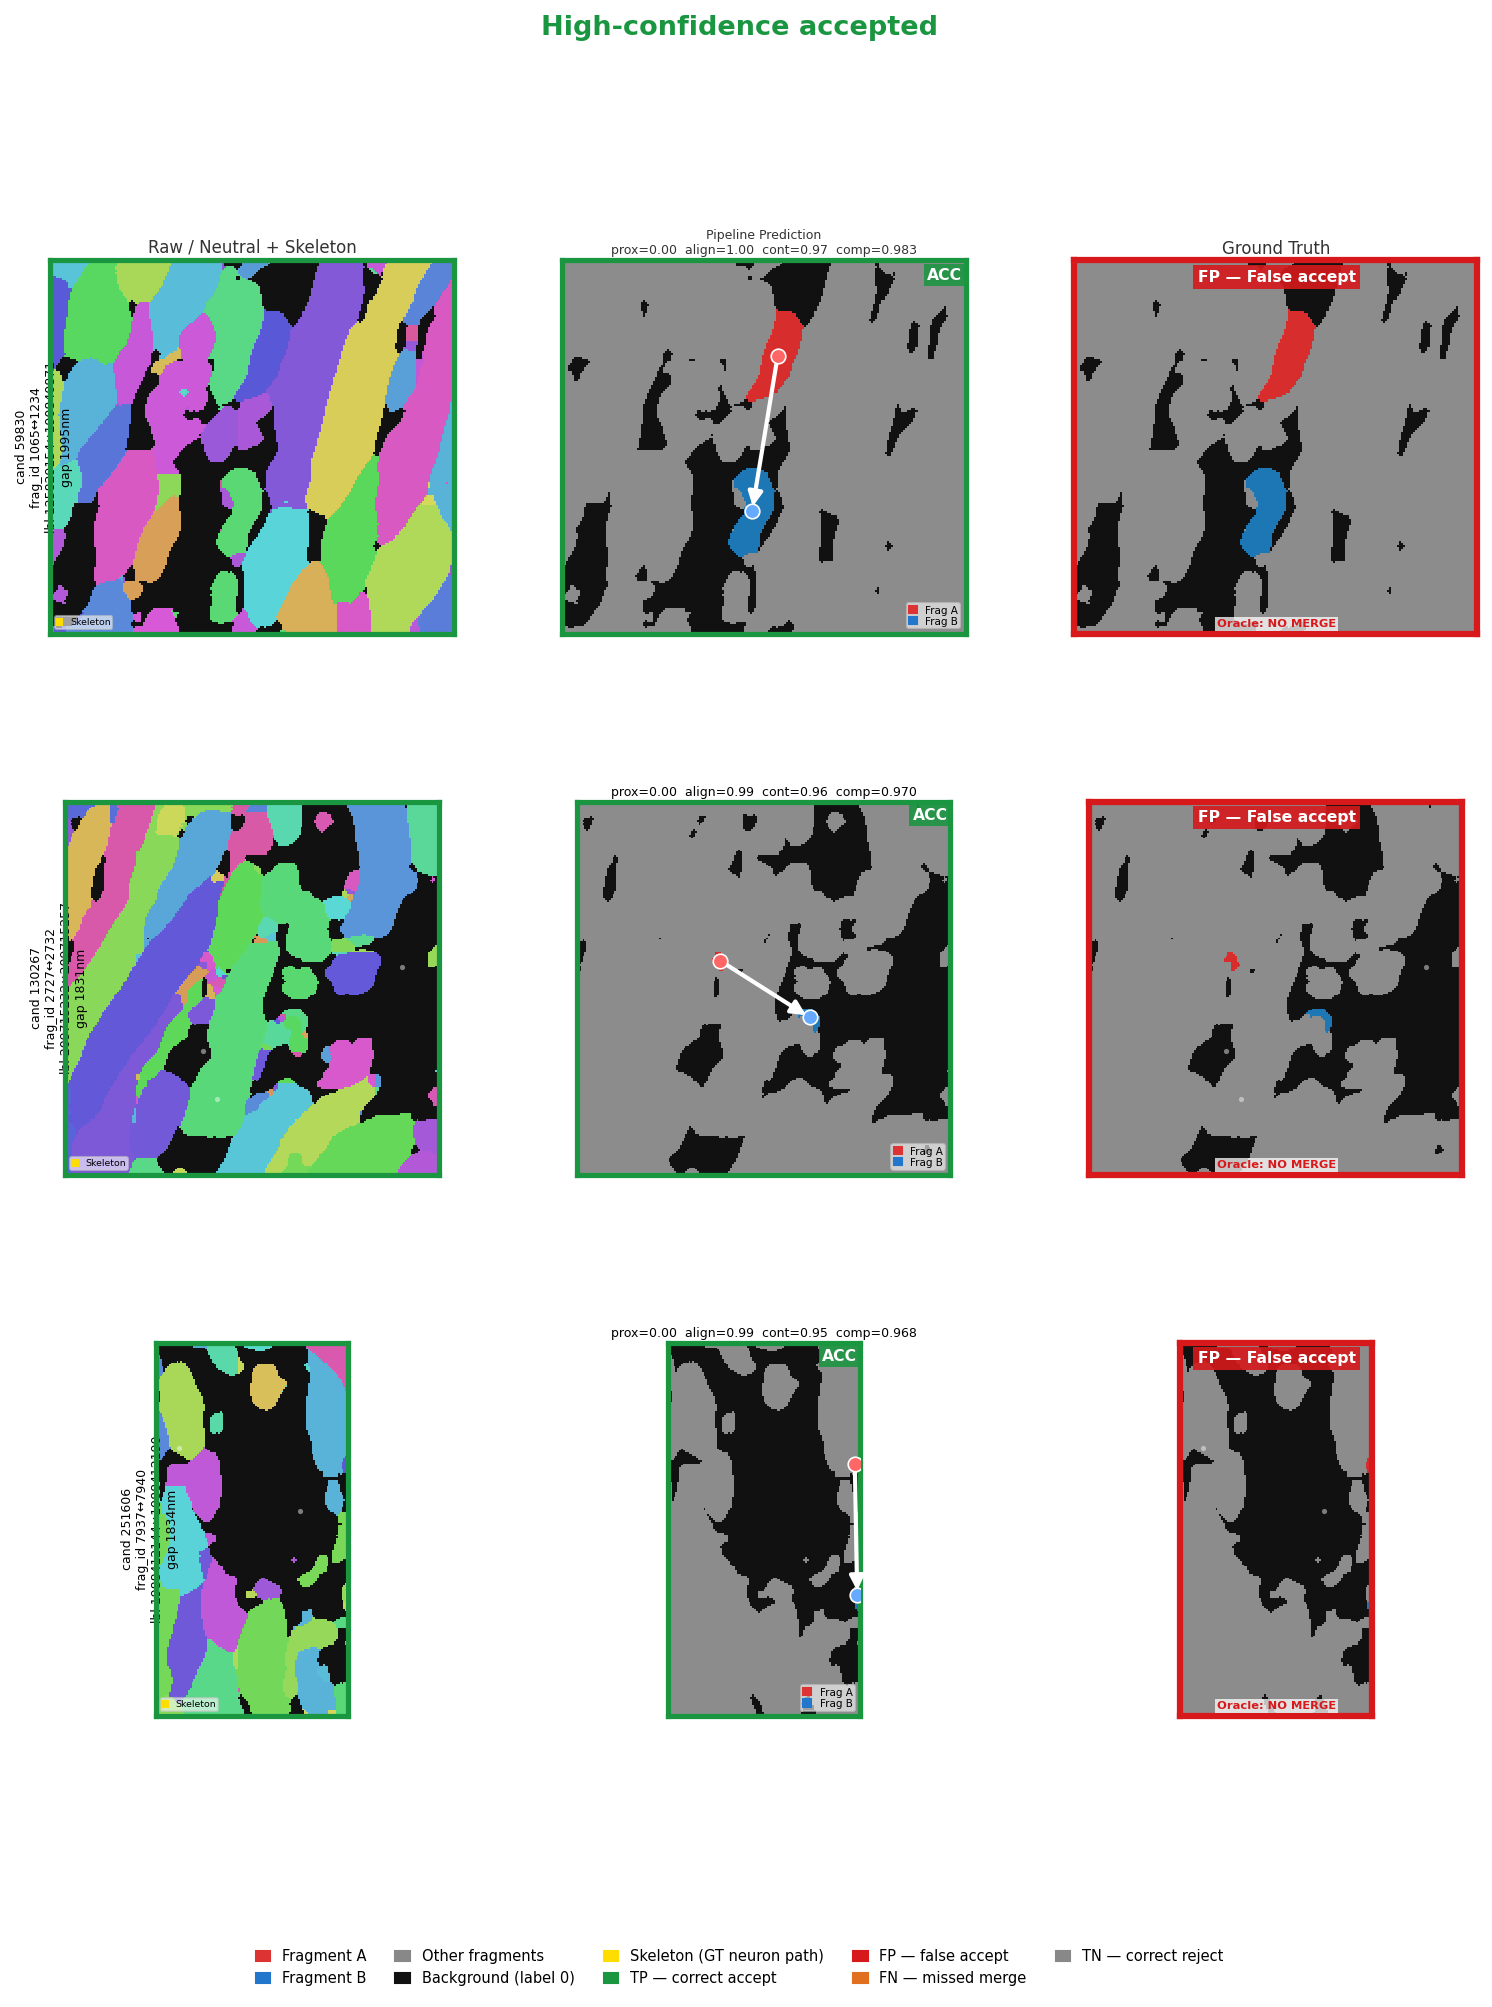
\includegraphics[width=\textwidth,height=0.78\textheight,keepaspectratio]{candidate_showcase_accepted.png}
  \caption{High-confidence accepted candidates (highest composite scores among
  accepted, non-same-label connections) from the XPRESS training volume.
  \textbf{Left (Panel~1):} Neutral segmentation with distinct muted colors per
  segment; yellow dots/lines show ground-truth skeleton nodes near the Z-slice.
  \textbf{Center (Panel~2):} Fragment~A in red, Fragment~B in blue, with the
  proposed connection arrow (ACC badge) and all five component scores.
  \textbf{Right (Panel~3):} Ground-truth verdict (TP/FP/FN/TN badge); bright yellow
  skeleton highlights the neurons passing through both fragments, with a dashed
  line marking ground-truth-positive edge crossings. The FP outcomes for these candidates
  reflect the low precision of the pipeline at this operating point: with
  ${\sim}368{,}000$ accepted candidates and only ${\sim}1{,}494$ true positives,
  even geometrically compelling pairs are predominantly false accepts.  The
  visual report makes this trade-off immediately visible.}
  \label{fig:accepted}
\end{figure}

\begin{figure}[htbp]
  \centering
  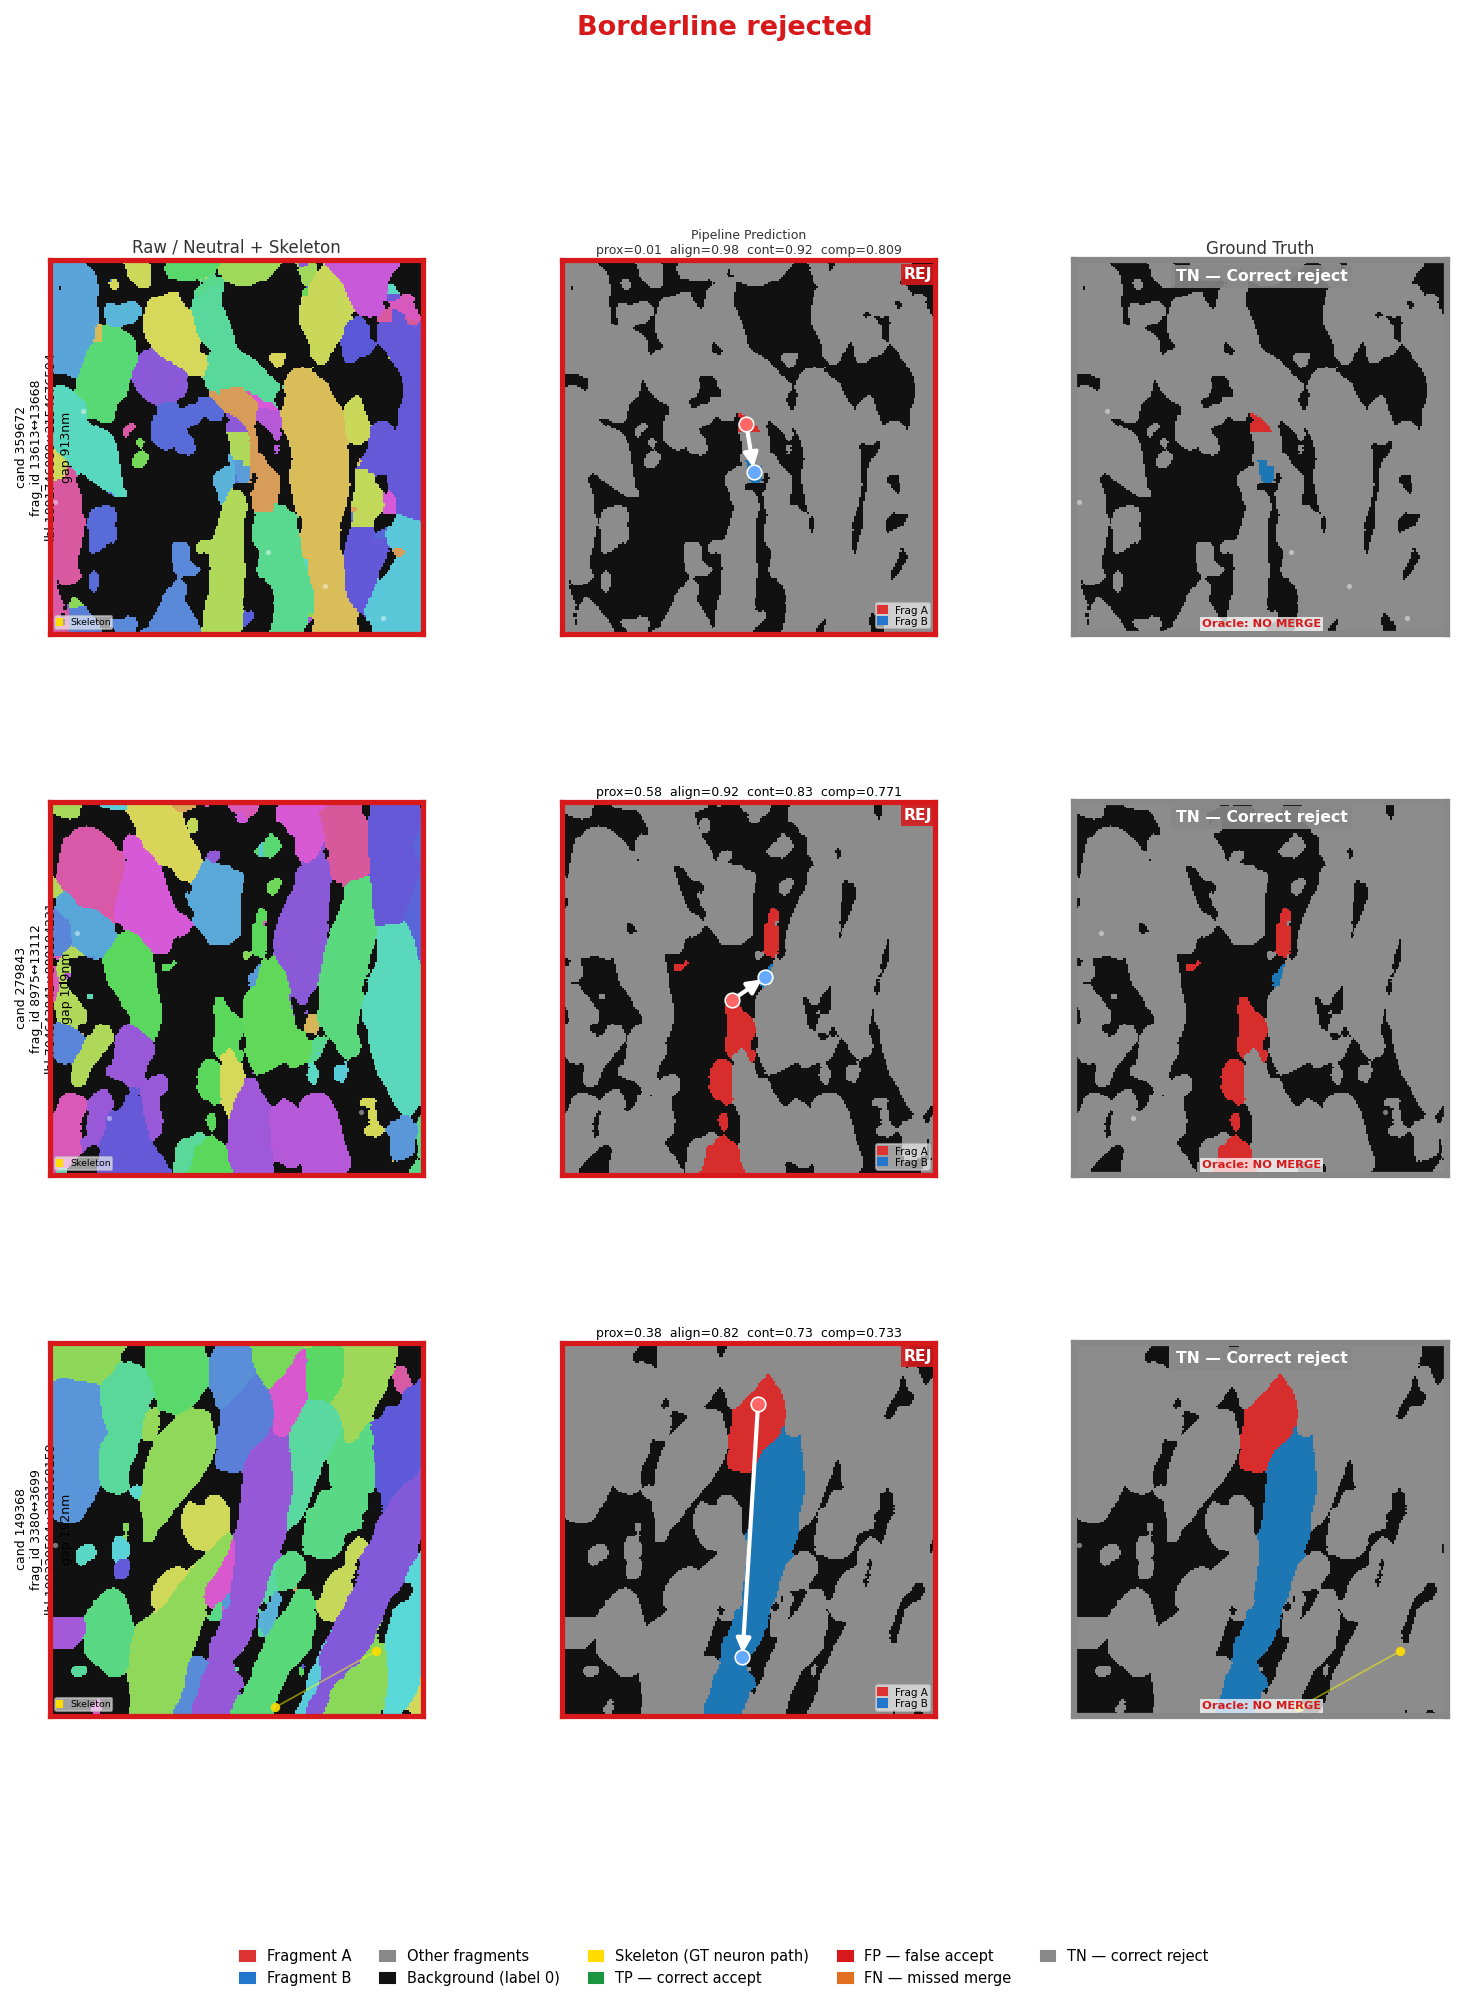
\includegraphics[width=\textwidth,height=0.78\textheight,keepaspectratio]{candidate_showcase_rejected.png}
  \caption{Borderline rejected candidates (highest composite scores among all
  rejected, non-same-label connections).  These are the cases the pipeline
  declines to merge while scoring closest to acceptance.  All three shown are
  TN (correct rejections): the ground truth confirms no skeleton crossing between the
  two fragments, consistent with the pipeline's decision.  The skeleton overlay
  in Panel~1 makes the absence of a crossing evident: the ground-truth axon
  paths run through each fragment independently without bridging the gap.}
  \label{fig:rejected}
\end{figure}

The accepted panels (Figure~\ref{fig:accepted}) reveal an important characteristic
of the pipeline's operating regime: the composite score is optimised for recall,
not precision.  At the validation threshold used in Experiment~24, the pipeline
accepts ${\sim}368{,}000$ candidates to achieve ${\sim}0.996$ recall on the
$1{,}499$ ground-truth pairs, a design choice that requires a downstream filtering
step (e.g., the ML filter from Experiment~20) for deployment scenarios where
precision matters.  The borderline rejected panels (Figure~\ref{fig:rejected})
confirm that the rejection decisions are consistent with the geometric evidence:
cases where alignment and continuity scores are high but the ground truth confirms
no true split error exist.

\paragraph{Ground-truth TP inspection (end-to-end validation).}
Through Experiment~25 all evaluation was metric-driven (coverage, recall,
precision).  The ground-truth TP sampling category described in
Section~\ref{sec:visual-validation} closes this loop by filtering to the
intersection of pipeline-accepted and ground-truth-positive candidates and
asking, for each sampled row, whether the proposed merge is anatomically
real.  Running the inspection on the Experiment~24 training output (top
five ground-truth TPs by composite score, written to
\texttt{docs/visual\_report\_tp\_inspection.pdf}) confirmed that each
inspected TP is a genuine biological split: the ground-truth skeleton
visibly traverses both fragments, the fragments are morphologically
continuous across the gap, and the skeleton overlay in Panel~3 occupies
both label regions with a dashed ground-truth-positive indicator.  This is
the final non-automated layer of end-to-end validation and should be
re-run after any change that alters accepted-candidate composition.

\section{Gap-Stratified Precision Analysis}
\label{sec:gap-stratified}

The aggregate XPRESS precision of $\approx$0.003 on the Experiment~24 training
output is a single number that conceals large structural heterogeneity.  To
localize where the precision problem lives, we partitioned the 369{,}570
candidates into gap-distance bins and recomputed per-bin precision, recall,
and candidate volume using the same skeleton-edge-crossing ground-truth
construction described in Chapter~\ref{ch:methodology}.  This analysis is a
pure post-processing pass over the existing \texttt{connections.csv} export;
no pipeline re-run was required.  The analysis script is reproducible at
\texttt{scripts/gap\_stratified\_precision.py}.  Results are summarized in
Table~\ref{tab:gap_stratified} and Figure~\ref{fig:gap_stratified}.

\begin{table}[H]
\centering
\caption{Per-bin precision/recall on the Experiment~24 training volume.  ``TP''
and ``FP'' are candidate-level counts (each accepted candidate contributes
independently).  ``Candidates'' is total generated (accepted $+$ rejected)
within the bin.  Precision is computed from candidate counts; recall from
covered ground-truth pairs within the bin.  Note: the candidate-level TP total
of 1{,}248 differs from the 1{,}175 ``unique GT merge pairs accepted'' figure
reported in Table~\ref{tab:xpress_best} because a single ground-truth pair can
appear as multiple distinct accepted candidates (e.g., when several skeleton
edges of the same axon cross the fragment boundary).  Both accountings
describe the same underlying run.}
\label{tab:gap_stratified}
\small
\begin{tabular}{@{}lrrrrr@{}}
\toprule
Gap bin (nm) & Candidates & TP & FP & Precision & Recall \\
\midrule
$[0, 100)$       & 3{,}675    & 25    & 3{,}636     & 0.0068 & 0.96 \\
$[100, 200)$     & 3{,}352    & 44    & 3{,}283     & 0.0132 & 1.00 \\
$[200, 300)$     & 6{,}261    & 125   & 6{,}090     & 0.0201 & 0.99 \\
$[300, 500)$     & 20{,}418   & 594   & 19{,}745    & \textbf{0.0292} & 1.00 \\
$[500, 750)$     & 1{,}720    & 11    & 1{,}663     & 0.0066 & 1.00 \\
$[750, 1000)$    & 8{,}670    & 35    & 8{,}021     & 0.0043 & 0.95 \\
$[1000, 1500)$   & 52{,}062   & 117   & 51{,}936    & 0.0022 & 1.00 \\
$[1500, 2000)$   & \textbf{222{,}788} & 203 & \textbf{222{,}572} & 0.0009 & 1.00 \\
$[2000, 3000)$   & 1{,}902    & 32    & 1{,}856     & 0.0169 & 1.00 \\
$[3000, 20000)$  & 48{,}720   & 62    & 48{,}131    & 0.0013 & 1.00 \\
\midrule
Total            & 369{,}570  & 1{,}248 & 366{,}933 & 0.0034 & 0.9960 \\
\bottomrule
\end{tabular}
\end{table}

\begin{figure}[H]
\centering
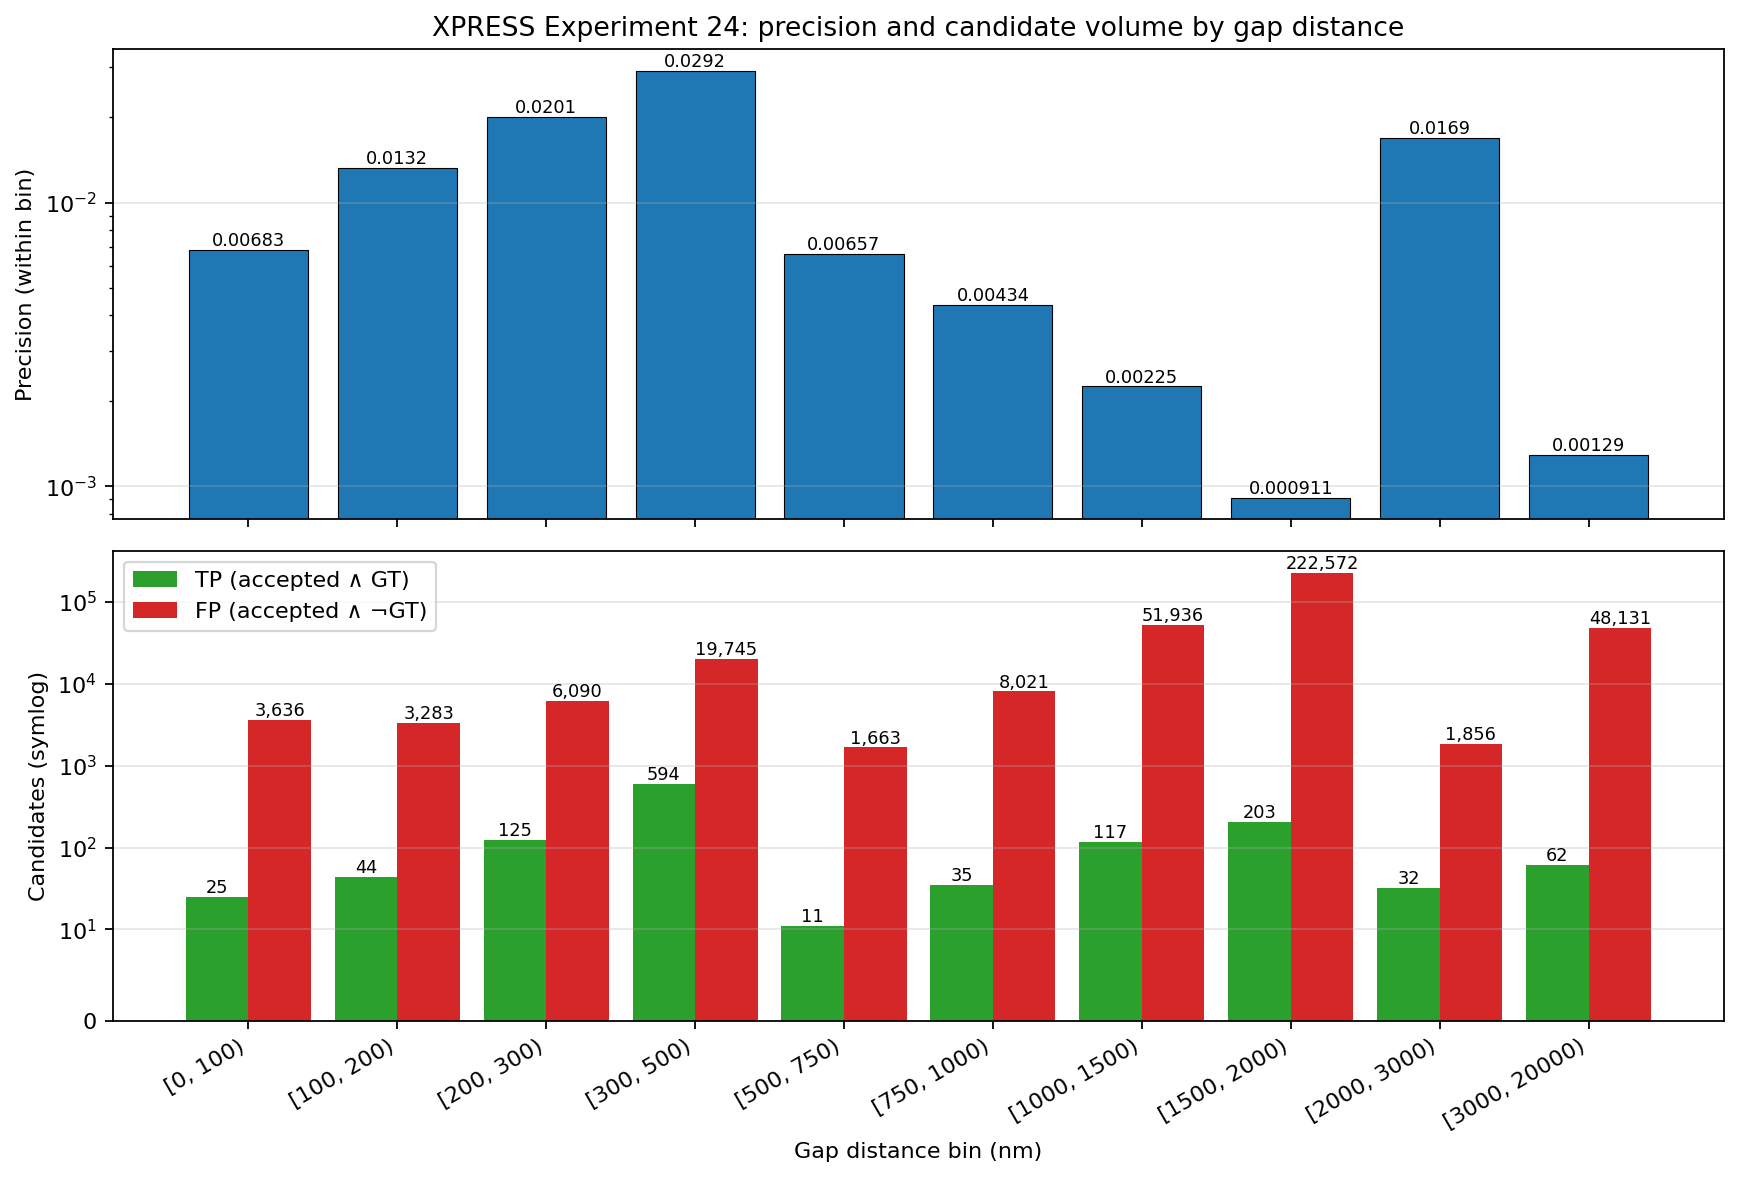
\includegraphics[width=\textwidth]{gap_stratified_precision.png}
\caption{XPRESS Experiment~24 per-bin analysis. \textbf{Top:} in-bin precision
on a log scale, peaking at 0.029 in the $[300, 500)$~nm bin (about $10\times$
the overall figure) and collapsing to 0.0009 in the $[1500, 2000)$~nm bin.
\textbf{Bottom:} true-positive (green) and false-positive (red) candidate
counts per bin on a symlog scale. The $[1500, 2000)$~nm bin alone accounts for
60.7\% of all false positives (222{,}572 of 366{,}933) while contributing
only 16.3\% of true positives.}
\label{fig:gap_stratified}
\end{figure}

\paragraph{Findings.}
Three structural observations emerge:

\begin{enumerate}
  \item \textbf{Short-gap precision is an order of magnitude higher.}
        The $[100, 500)$~nm bins achieve precision 0.013--0.029, compared to
        the overall 0.003.  These gap sizes correspond to genuine interior
        skeleton-node splits where the two fragments are close enough that
        alignment and continuity scores are informative.

  \item \textbf{Long-range pairs dominate the FP budget.}
        The $[1000, 2000)$~nm range --- the regime where the distance-conditioned
        weight vector is active --- contains 74.4\% of all candidates
        (274{,}850 / 369{,}570) and 74.8\% of all false positives
        (274{,}508 / 366{,}933), but only 25.6\% of true positives
        (320 / 1{,}248).  The long-range pass pays a precision price that
        short-range scoring does not.

  \item \textbf{Precision rebounds at $[2000, 3000)$~nm}
        (0.017, second-highest of all bins) because these candidates are rare
        (1{,}902 total) and most arise from PCA-endpoint pairings on large
        fragments, where the bbox-tip estimate is only informative for
        genuine long axon splits.  Above 3{,}000~nm, spurious PCA pairings
        dominate and precision drops again.
\end{enumerate}

\paragraph{Generalization to validation volume.}
Running the same post-processing on the Experiment~24 held-out validation
output reproduces the same shape: the $[300, 500)$~nm bin is the precision
peak (0.0025) and the $[1500, 2000)$~nm bin alone contains 65.5\% of all
false positives (300{,}763 / 458{,}941).  The absolute precision numbers
are lower on validation because there are fewer ground-truth pairs per
candidate (203 vs.\ 1{,}499), but the relative ordering across bins is
preserved.  This confirms that the precision-by-gap structure is a
property of the XPRESS domain (white matter axon density at long range),
not an artifact of training-volume tuning.

\paragraph{Implications for future precision work.}
Three directions follow directly from the per-bin decomposition:

\begin{itemize}
  \item A gap-dependent accept threshold --- looser at $[100, 500)$~nm, much
        stricter at $[1000, 2000)$~nm --- would retain most TPs while cutting
        most FPs.  The $[300, 500)$~nm bin retains 594 TPs at precision 0.029
        with a uniform threshold; moving the $[1500, 2000)$~nm threshold up
        to discard its 222{,}572 FPs would cost at most 203 TPs.
  \item The machine-learned filter of Experiment~20 should be retrained
        stratified by gap, since the feature distribution and operating
        point differ sharply between bins.
  \item Reducing \texttt{max\_endpoint\_search\_nm} from 2000 to 1000~nm is
        worth re-testing.  Experiment~13 (3000~nm) was rejected for recall
        regression, but the reverse direction --- tightening to 1000~nm ---
        would discard the long-range bins entirely, lose the 117 TPs at
        $[1000, 1500)$~nm and 203 at $[1500, 2000)$~nm (25.6\% of total TPs),
        and save $\sim$270{,}000 FPs.  This would yield recall near 0.73
        at precision $\approx$0.015, a substantially different operating
        point that may be preferable when precision matters more than
        absolute recall.
\end{itemize}

\section{Neighborhood-Density Re-ranker}
\label{sec:density-reranker}

The per-bin analysis (Section~\ref{sec:gap-stratified}) localizes the
precision problem to the long-range regime but does not explain why one
long-range candidate is a true split and another is not.  A natural
hypothesis --- motivated by the direction-weighted scoring story of
Experiment~24 --- is that a genuine same-axon split pair is
\emph{locally isolated}: its axon is the primary structure in the
neighborhood.  A cross-axon false positive sits in a crowd of other axons
that makes many geometrically-plausible alternatives to the pipeline's
chosen partner.  A simple count of other fragments in the neighborhood
of the candidate should therefore separate TPs from FPs even after the
composite score has already accepted both.

This section tests that hypothesis as a post-hoc re-ranker on the
Experiment~24 accepted-candidate set.  The analysis script
(\texttt{scripts/neighborhood\_density\_reranker.py}) is pure
post-processing: no pipeline code or pipeline configuration is modified.

\paragraph{Feature definition.}
For each accepted candidate with fragments $a$ and $b$:
\begin{align*}
\text{mid}    &= (\text{centroid}_a + \text{centroid}_b) / 2 \\
\text{density\_mid}(R) &= \big|\{\,c : c \neq a, b \text{ and } \|\text{centroid}_c - \text{mid}\| \le R\,\}\big| \\
\text{density\_max}(R) &= \max\left(|\mathcal{N}_R(a)|,\, |\mathcal{N}_R(b)|\right) - 2
\end{align*}
where $\mathcal{N}_R(f)$ is the set of fragment centroids within radius $R$
of fragment $f$'s centroid.  We evaluated $R \in \{500, 1000, 1500, 2000, 3000\}$~nm;
$R = 1500$~nm gave the best precision-at-recall scores and is used in the
figures below.

\paragraph{Distribution of the feature.}
Figure~\ref{fig:density-distribution} shows the per-candidate density
distributions stratified by ground-truth status.  The TP distribution is
visibly shifted toward lower density: for \texttt{density\_mid\_1500}, TP
mean is 9.6 vs FP mean 13.4; for \texttt{density\_max\_1500}, TP mean is
12.1 vs FP mean 15.6.  The two distributions overlap substantially but
the means are distinct, confirming the qualitative hypothesis.

\begin{figure}[H]
\centering
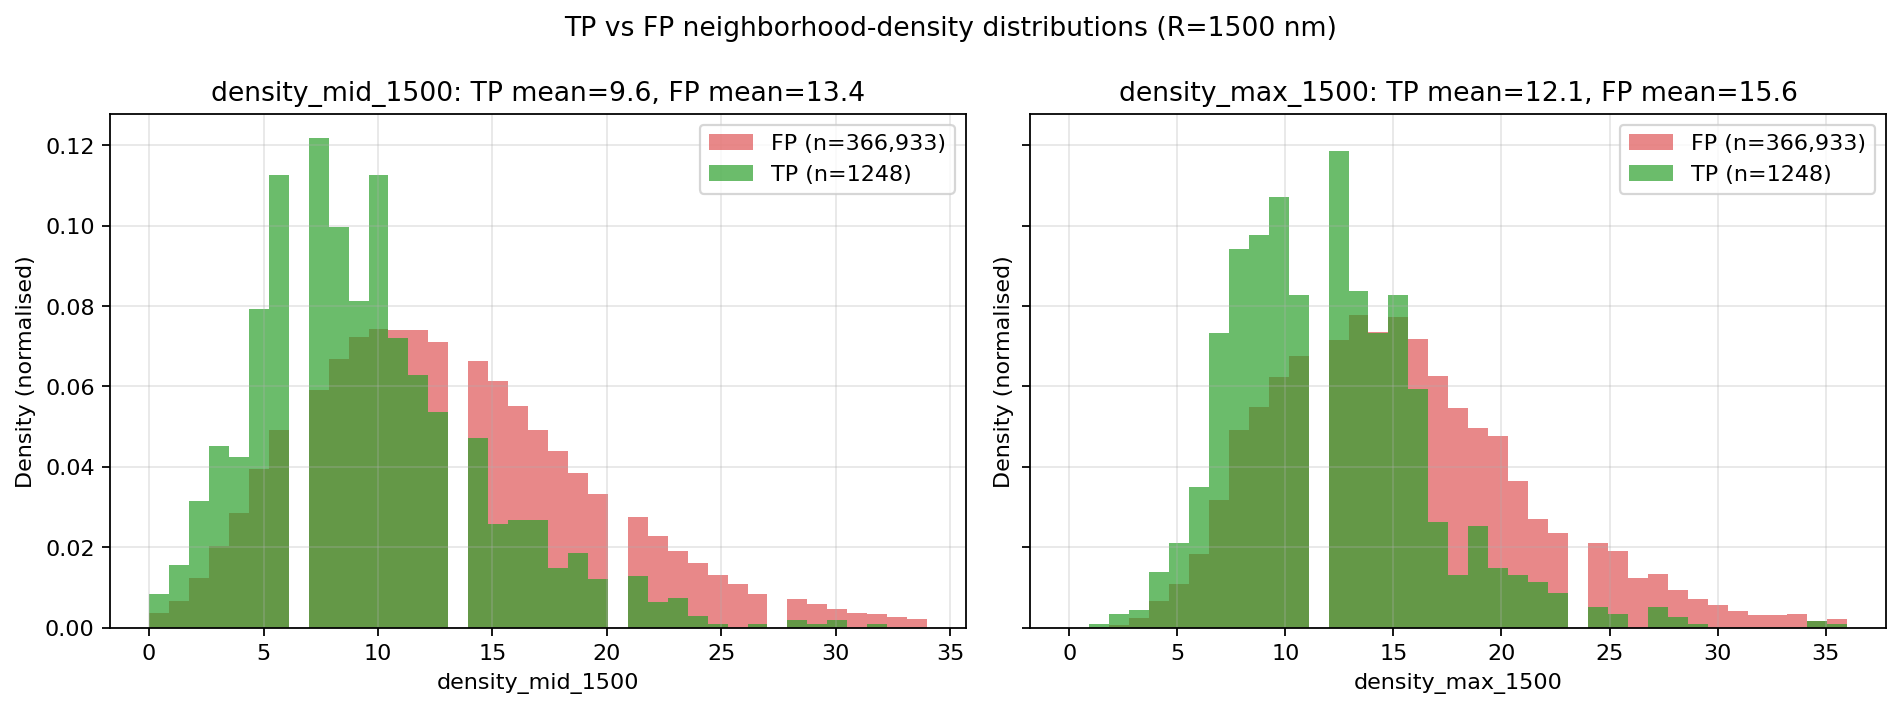
\includegraphics[width=\textwidth]{density_distribution.png}
\caption{Neighborhood-density feature distributions for the 368{,}181
Experiment~24 accepted candidates, stratified by ground-truth status
(TP = accepted $\land$ GT-positive, FP = accepted $\land$ $\neg$GT).
\textbf{Left:} \texttt{density\_mid\_1500} (count of fragment centroids
within 1{,}500~nm of the candidate midpoint). \textbf{Right:}
\texttt{density\_max\_1500} (max of the per-fragment counts). The TP
distribution is shifted toward lower density in both cases.}
\label{fig:density-distribution}
\end{figure}

\paragraph{Re-ranker performance.}
Table~\ref{tab:density-reranker} reports precision at fixed recall
targets for three ranking strategies: the baseline composite score
(descending), the density features alone (ascending), and a combined
score that adds $\alpha \log(1 + \text{density\_mid})$ as a penalty
term.  The composite-score baseline within the already-accepted set is
remarkably uninformative --- precision varies by less than 3\% across
the 0.85--0.99 recall range --- reflecting that all accepted candidates
occupy a narrow composite-score band by construction.  The density
features provide a genuine if modest improvement at mid-recall,
reaching a 49\% relative gain at recall $0.85$.

\begin{table}[H]
\centering
\caption{Precision at fixed recall targets on Experiment~24 accepted
candidates (training volume).  Numbers in parentheses show the validation
volume.  ``Rel.'' is the relative improvement of
\texttt{density\_max\_1500} over the composite-score baseline on training.}
\label{tab:density-reranker}
\small
\begin{tabular}{@{}lrrrr@{}}
\toprule
Recall & Composite baseline & density\_mid\_1500 & density\_max\_1500 & Rel. \\
\midrule
0.99 & 0.0034 \,(0.00038) & 0.0036 \,(0.00040) & 0.0035 \,(0.00040) & $+$4\% \\
0.95 & 0.0034 \,(0.00038) & 0.0039 \,(0.00042) & 0.0039 \,(0.00045) & $+$15\% \\
0.90 & 0.0034 \,(0.00038) & 0.0043 \,(0.00044) & 0.0045 \,(0.00054) & $+$33\% \\
0.85 & 0.0033 \,(0.00037) & 0.0048 \,(0.00048) & 0.0049 \,(0.00056) & $+$49\% \\
\bottomrule
\end{tabular}
\end{table}

\begin{figure}[H]
\centering
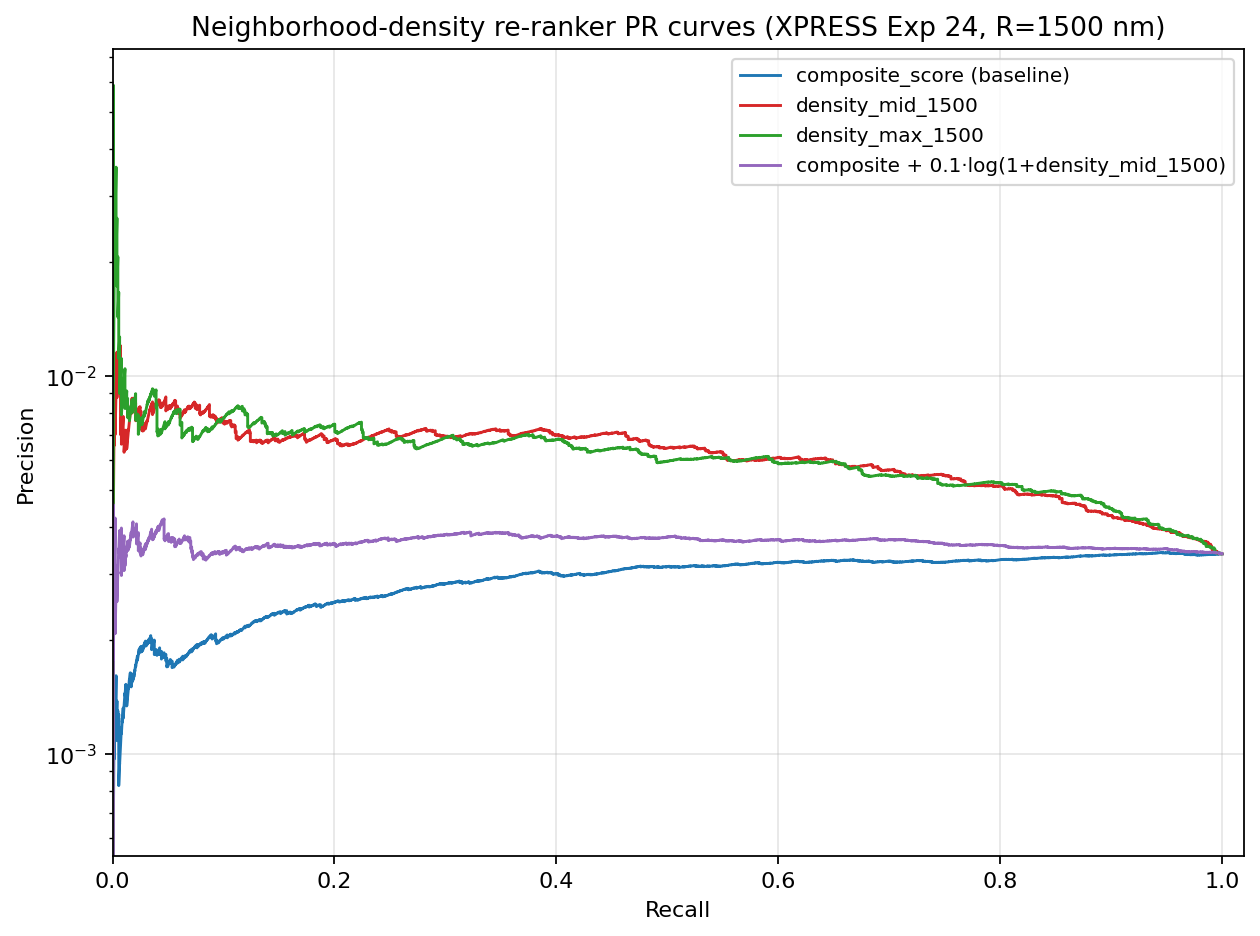
\includegraphics[width=0.92\textwidth]{density_pr_curve.png}
\caption{Precision-recall curves on the 368{,}181 Experiment~24 accepted
candidates for four ranking strategies: composite score (blue, baseline),
density\_mid\_1500 (red), density\_max\_1500 (green), and a combined
score composite $+ 0.1 \log(1 + \text{density\_mid\_1500})$ (purple).
Density features dominate the baseline across the 0.2--0.95 recall
range.  Note the log-scale on precision.  All curves converge at
recall $=1$, where every accepted candidate is kept and precision is
the aggregate 0.0034.}
\label{fig:density-pr}
\end{figure}

\paragraph{Findings.}

\begin{enumerate}
  \item \textbf{The hypothesis is empirically confirmed.}  Accepted-candidate
        density distributions differ between TP and FP populations
        (TP mean $\approx 25\%$ lower than FP mean at $R=1500$~nm), and a
        density-only re-ranker improves precision over composite-score
        re-ranking by up to 49\% at recall 0.85.

  \item \textbf{The effect decays sharply at high recall.}  At recall 0.99
        the improvement is only 4--6\% in both training and validation,
        because the $\sim$1\% of TPs that are hardest to recover have density
        indistinguishable from the FP background.  Density alone does not
        break the geometric-features precision ceiling at the recall target
        where the pipeline currently operates.

  \item \textbf{Composite score is not a useful re-ranker for already-accepted
        candidates.}  Its PR curve within the accepted set is nearly flat at
        precision $\approx 0.003$ across the full recall range
        (Figure~\ref{fig:density-pr}).  All accepted candidates have, by
        construction, composite scores above the acceptance threshold, and
        within that band score magnitude carries little signal about
        ground-truth status.

  \item \textbf{Density is complementary, not redundant, with the degree
        feature of Experiment~20.}  The ML filter of Experiment~20 achieved
        precision 0.037 at recall 0.85 using per-fragment degree.  Density
        at recall 0.85 achieves only 0.005 on its own --- an order of
        magnitude weaker --- but the two features encode different signals
        (how many partners has this fragment been paired with vs.\ how
        crowded is the local neighborhood).  The combined composite + density
        score (purple curve) does \emph{not} beat density alone in our
        experiments, because composite is a pure noise term on this slice;
        a learned combination with the degree feature is expected to do
        better and is left for future work.

  \item \textbf{Validation reproduces the pattern.}  On the held-out
        validation volume, the same relative improvement ordering holds
        (+6\% at recall 0.99, +50\% at recall 0.85), confirming that
        density is a real signal in this domain rather than a
        training-set artifact.
\end{enumerate}

\paragraph{Implication.}
The neighborhood-density feature is a worthwhile addition to any future
learned post-filter but is insufficient as a standalone precision
recovery strategy at recall $\geq 0.99$.  This is consistent with the
overall narrative of the XPRESS precision challenge: no single
geometric signal separates same-axon from cross-axon pairs at the
density of myelinated white matter, and meaningful precision gains at
high recall will require either multi-feature ML (retrained on features
including density) or access to raw image data.

\section{Per-Bin Threshold Precision Ceiling}
\label{sec:per-bin-threshold}

Sections~\ref{sec:gap-stratified} and~\ref{sec:density-reranker}
characterized the precision problem and attempted a single-feature
remedy.  A natural follow-up question is: \emph{what is the best
precision any pipeline variant can achieve if its only degree of
freedom is a per-gap-bin composite threshold?}  This sets an empirical
ceiling on all gap-aware threshold-tuning strategies --- including
the gap-dependent accept thresholds suggested by Section~\ref{sec:gap-stratified}
and any future ML filter whose inputs are limited to the current
geometric scores plus gap bin.  Quantitative results are summarized in
Table~\ref{tab:per-bin-threshold} and the full PR frontier is shown
in Figure~\ref{fig:per-bin-threshold}.

\paragraph{Method.}
For each accepted candidate we know the gap bin, the composite score,
and the ground-truth label.  The per-bin ceiling is constructed
by sorting candidates within each gap bin by composite score
(descending) and then merging the per-bin streams greedily: at each
step, whichever bin has a ground-truth positive at its next pointer
contributes that candidate for free; when no such bin exists, the bin
with the highest remaining TP-density (remaining TPs / remaining
candidates) contributes its next candidate.  This produces a global
PR curve that is the upper envelope across all per-bin
threshold-assignment strategies.  The construction uses ground-truth
labels to determine the merge order, so it represents an upper bound;
any learnable per-bin policy will sit on or below this curve.

\begin{table}[H]
\centering
\caption{Precision at fixed recall targets for the global composite
threshold (Experiment~24 baseline) vs the per-bin ground-truth ceiling.
Numbers in parentheses are the held-out validation volume.
``Rel.~gain'' is the relative precision improvement of per-bin vs
global on the training volume.}
\label{tab:per-bin-threshold}
\small
\begin{tabular}{@{}lrrr@{}}
\toprule
Recall & Global baseline & Per-bin ceiling & Rel.~gain \\
\midrule
0.99 & 0.0034 \,(0.00038) & 0.0034 \,(0.00041) & $+$1.3\% \\
0.95 & 0.0034 \,(0.00038) & 0.0040 \,(0.00055) & $+$16.4\% \\
0.90 & 0.0034 \,(0.00038) & 0.0051 \,(0.00087) & $+$50.6\% \\
0.85 & 0.0033 \,(0.00037) & 0.0068 \,(0.00104) & $+$104\% \\
0.80 & 0.0033 \,(0.00037) & 0.0085 \,(0.00143) & $+$161\% \\
0.70 & 0.0032 \,(0.00035) & \textbf{0.0169} \,(\textbf{0.00303}) & $+$421\% \\
\bottomrule
\end{tabular}
\end{table}

\begin{figure}[H]
\centering
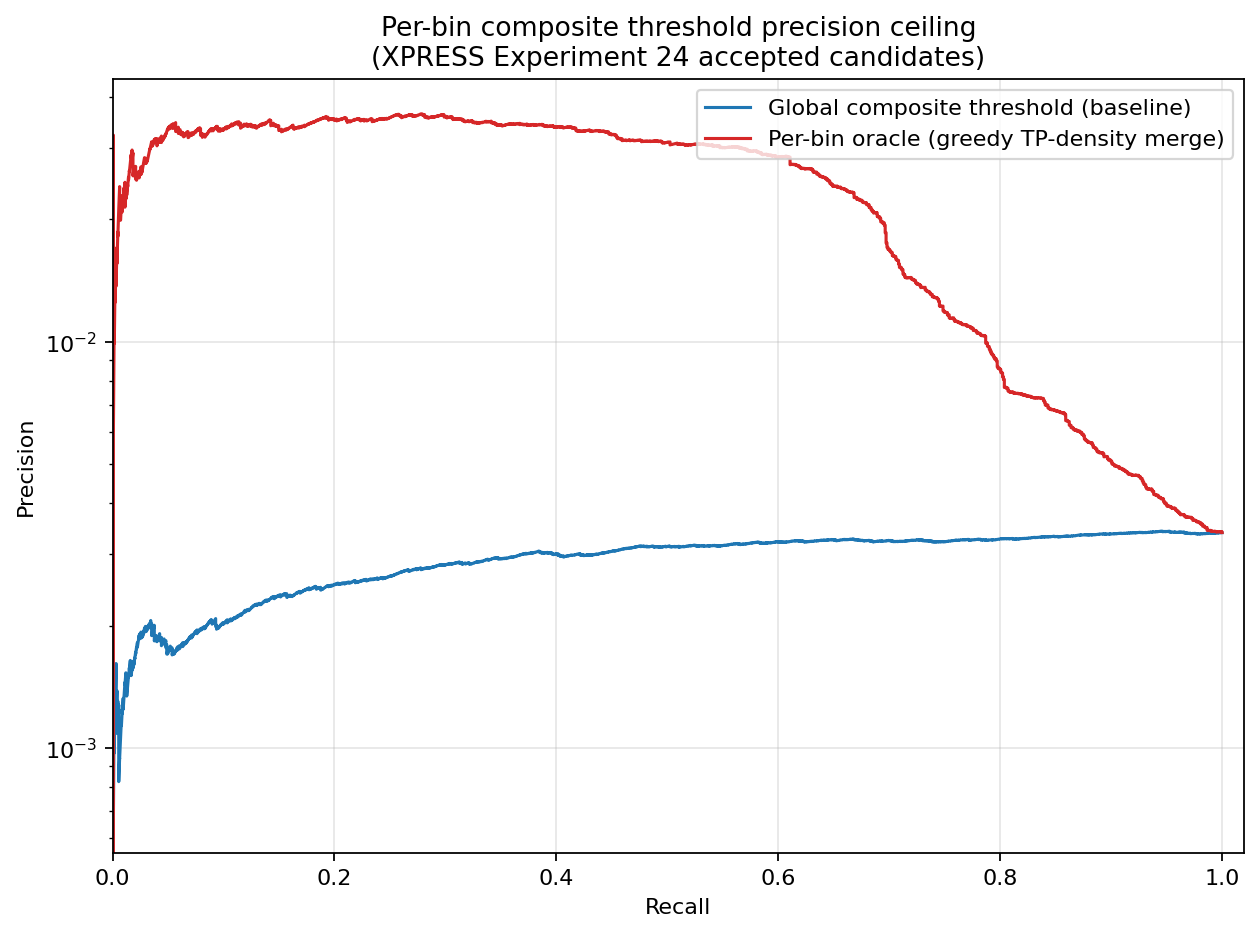
\includegraphics[width=0.92\textwidth]{per_bin_threshold_pr.png}
\caption{Precision-recall frontier for the two strategies on the
Experiment~24 accepted-candidate set.  \textbf{Blue:} the global
composite threshold (the baseline behavior of Experiment~24 after the
fact) is nearly flat at precision $\approx 0.003$ across the full
recall range.  \textbf{Red:} the per-bin ground-truth ceiling reaches
$\sim$4\% precision at low recall and holds above 1\% up to recall
$\approx 0.80$ before collapsing to meet the baseline at recall 1.
The two curves converge at recall $1$ where every accepted candidate
is kept.  Log-scale precision.}
\label{fig:per-bin-threshold}
\end{figure}

\paragraph{Findings.}

\begin{enumerate}
  \item \textbf{The recall-0.99 ceiling is nearly flat.}  At recall 0.99
        the per-bin ceiling gains only 1.3\% over the global baseline
        (9\% on validation).  The hardest-to-recover 1\% of TPs are
        scattered across the same bins that hold the bulk of the FPs, so
        no per-bin threshold allocation can cut FPs meaningfully without
        sacrificing those TPs.  This explains why Experiment~20's ML
        filter could not maintain recall $\geq 0.99$ with meaningful
        precision improvement: the ceiling is intrinsic to the
        geometric feature space plus gap bin, not an ML-architecture
        shortcoming.

  \item \textbf{The recall-$\leq 0.90$ ceiling is substantially higher.}
        At recall 0.90, per-bin thresholding can reach 0.005 precision
        ($+51\%$); at recall 0.85, 0.007 ($+104\%$); at recall 0.70,
        0.017 ($+421\%$).  These are the operating points at which
        per-bin threshold tuning becomes a meaningful deployment lever.

  \item \textbf{Validation reproduces the structure.}  On the held-out
        volume the absolute precision numbers are lower, but the
        relative gain ordering is preserved: +9\% at recall 0.99 rising
        to +773\% at recall 0.70.

  \item \textbf{Comparing to alternative precision strategies.}
        Experiment~20's ML filter reached precision 0.037 at recall
        0.85.  The per-bin ceiling at recall 0.85 is 0.007 --- 5x
        lower --- meaning Experiment~20's degree-feature signal gave
        access to information beyond what any gap-aware threshold
        strategy can capture.  Conversely, the density re-ranker of
        Section~\ref{sec:density-reranker} peaked at 0.005 at recall
        0.85, which is close to the per-bin ceiling: density
        plus gap captures nearly all the gap-bin-aware precision
        signal, and further gains require orthogonal features such
        as per-fragment degree or raw-image evidence.
\end{enumerate}

\paragraph{Implication.}
Per-bin threshold tuning is a concrete, low-risk deployment lever at
recall $\leq 0.90$ but delivers essentially nothing at recall 0.99.
Any future work targeting high-recall precision must combine
orthogonal feature classes (per-fragment degree, neighborhood density,
skeleton-morphology features, or raw image evidence) rather than
merely redistributing the existing composite score.  This result
constrains the design of the recommended multi-feature gap-stratified
ML filter (Chapter~\ref{ch:futurework}): a useful model must move
decisions outside the convex hull set by composite-plus-gap, not simply
calibrate within it.

\section{Test Coverage}

The pipeline is validated by 428 automated tests across 20 test modules,
covering all pipeline stages, configuration loading, export formats, and edge
cases. All tests pass on Python 3.10, 3.11, and 3.12. Continuous integration
via GitHub Actions runs tests, black formatting checks, and mypy type checks on
every push.

\begin{table}[H]
\centering
\caption{Test suite summary.}
\label{tab:tests}
\begin{tabular}{@{}lr@{}}
\toprule
Module & Tests \\
\midrule
I/O readers & 22 \\
Fragment extraction & 35 \\
Graph construction & 18 \\
Candidate generation \& scoring & 40 \\
Validation rules & 85 \\
Assembly & 35 \\
Export formats & 50 \\
Ground truth evaluation & 30 \\
ML filter & 28 \\
Visualization & 12 \\
Configuration & 28 \\
End-to-end pipeline & 12 \\
Other (CLI, logging, spatial math) & 33 \\
\midrule
\textbf{Total} & \textbf{428} \\
\bottomrule
\end{tabular}
\end{table}


\chapter{Related Work} \label{ch:relatedwork}
\section{Automated Neural Segmentation}

The dominant approach to large-scale neural segmentation uses convolutional
neural networks trained to predict affinities or boundary probabilities, followed
by a graph-based merge step (watershed, multicut, or similar) to produce
instance labels. Flood-filling networks (FFN)~\cite{januszewski2018high} achieve
state-of-the-art results on EM data by iteratively extending segment predictions
from seeds, and are used as the baseline segmenter for the XPRESS challenge.
PyTorch Connectomics~\cite{lin2021pytorch} provides a flexible framework for
training and deploying multiple segmentation architectures.

\section{Proofreading Infrastructure}

The CAVE (Connectome Annotation Versioning Engine)~\cite{dorkenwald2022cave}
system provides infrastructure for storing, versioning, and updating connectomics
annotations at scale. CAVE implements a chunk-based merge graph (PyChunkedGraph)
that allows atomic merge and split operations with full provenance tracking.
Our pipeline is designed to produce outputs compatible with CAVE-style
infrastructure: candidate connections in CSV form map naturally to proposed
merge operations, and the Neuroglancer annotation export can be overlaid in
CAVE's Neuroglancer integration.

The MICrONS Consortium~\cite{microns2025} recently published a functional
connectome of mouse visual cortex ($\sim$200{,}000 neurons, $\sim$500 million
synapses), representing the current scale of ambition for automated connectomics.
The proofreading pipeline underlying MICrONS relied on CAVE and extensive human
review, highlighting the importance of automated tools that reduce the human
burden.

\section{Error Detection and Correction}

Zung et al.~\cite{zung2017} proposed a framework for detecting and correcting
segmentation errors using a classifier trained on local volume patches. Their
approach operates at the voxel level, re-examining the raw image near putative
error sites. Our work operates entirely in the post-segmentation graph domain,
which is faster (no re-examination of raw data) and format-agnostic (works on
any segmentation, not only those for which raw data is available).

Plaza et al.~\cite{plaza2018analyzing} provide a rigorous treatment of
segmentation quality metrics for connectomics, including the definitions of
split and merge errors, the rand index, and the variation of information used
in challenge evaluations. Their framework informed the precision/recall
accounting used in this work, particularly the handling of ambiguous (AMBIGUOUS)
outcomes, which are excluded from precision/recall denominators.

\section{Skeleton-Based Proofreading}

Skeleton-based proofreading approaches identify potential split errors by
finding pairs of skeletons whose endpoints are spatially close and geometrically
compatible. Early systems used simple distance thresholds; modern approaches
add learned classifiers. The key contribution of this work is the skeleton-node
(interior) indexing strategy, which extends the detectable split positions from
fragment endpoints to any point along the axon.

The XPRESS challenge~\cite{xpress2023} was specifically designed to benchmark
automated proofreading of myelinated axons in XNH data, providing standardized
ground-truth oracle pairs for training and evaluation. To our knowledge, this
work is among the first applications of a conservative, rule-based graph-level
pipeline to the XPRESS benchmark, achieving Recall = 0.9958 on the training volume
and Recall = 0.9879 on the held-out validation volume.

\section{Graph Construction Strategies}

Several works have explored variants of the fragment graph construction problem.
Contact-based graphs (edges between touching fragments) are simple but miss
genuine splits with small gaps. Proximity-based graphs (edges between fragments
within a distance threshold) are more general; the key design choice is what
set of points to index. Our work systematically compares endpoint-only vs.\
full skeleton-node indexing and quantifies the impact of each on oracle coverage,
finding that full skeleton-node indexing is essential for interior splits.

The long-range endpoint pass introduced in Experiment~11 is similar in spirit
to approaches used in EM proofreading that specifically target ``broken wire''
errors by searching for endpoint pairs at larger radii than the standard
neighborhood. Our contribution is the distance-conditioned scoring that
accompanies this pass, preventing the proximity feature from suppressing
genuine long-range candidates.


\chapter{Conclusions} \label{ch:conclusion}
This work presents a conservative, modular post-segmentation pipeline for
automated split-error detection in connectomics data. The central research
question was: \emph{can a geometry-only, rule-based pipeline achieve high recall
on neural split detection without introducing excessive merge errors?}

On the CREMI Drosophila EM benchmark, the answer is clearly affirmative:
Precision = 1.000, Recall = 0.909, F1 = 0.952, with zero false positives. On
the XPRESS mouse white matter XNH challenge, a harder domain where the
segmented structures are elongated tubular axons with interior splits, the
best configuration (Experiment~24) achieves Recall = 0.9958 on the training
ground-truth set and Recall = 0.9879 on the fully held-out validation volume,
confirming generalization.

\paragraph{Key findings.}
Two innovations are responsible for the majority of the XPRESS recall improvement:

\begin{enumerate}
  \item The \textbf{skeleton-node graph} raises ground-truth coverage by 56.8
        percentage points over an endpoint-only graph in a single change, by
        enabling detection of interior splits along long axons.

  \item \textbf{Distance-conditioned scoring} prevents the proximity decay from
        suppressing long-range candidates whose alignment and continuity are
        strong, enabling the pipeline to accept splits at gaps up to 2000~nm.
\end{enumerate}

\paragraph{Challenges.}
The dominant open challenge is precision: Precision $\approx 0.003$ on XPRESS,
meaning approximately 312 false-positive merge proposals for every true positive.
The gap-stratified analysis in Section~\ref{sec:gap-stratified} localizes
this problem: the $[1500, 2000)$~nm bin alone contains 60.7\% of all false
positives while contributing only 16.3\% of true positives, and the
$[1000, 2000)$~nm long-range regime as a whole accounts for 74.8\% of
false positives at 25.6\% of true positives.  This stems from the geometric
feature space being insufficient to discriminate same-axon from cross-axon
long-range pairs at the density of myelinated white matter.  A machine-learned
filter (Experiment~20) improved precision $10\times$ (to 0.037) at the cost
of recall, but could not maintain recall $\geq 0.99$.  A neighborhood-density
re-ranker (Section~\ref{sec:density-reranker}) confirms that local crowding
is a real discriminator --- delivering up to 49\% relative precision gain at
recall 0.85 on both training and validation volumes --- but the effect
decays to $<$6\% at recall 0.99, showing that no single geometric signal
breaks the precision ceiling in this regime.  A per-bin ceiling analysis
(Section~\ref{sec:per-bin-threshold}) formalises this observation:
the precision ceiling achievable by any gap-aware threshold strategy
on the existing (composite, gap\_bin) feature pair is only $+$1.3\% at
recall 0.99 but rises to $+$104\% at recall 0.85 and $+$421\% at recall
0.70.  At recall 0.99 the hardest-to-recover TPs are distributed across
the same gap bins that hold the bulk of the FPs, so no per-bin
reallocation can remove FPs without sacrificing those TPs.  Meaningful
high-recall precision improvement therefore requires features
orthogonal to the current geometric scores (for example per-fragment
degree, as in Experiment~20) or access to raw image data.

The MinGapRule challenge was resolved in Experiment~24: disabling the rule
(min\_gap\_nm = 0) recovered all 37 short-gap false negatives and raised
training recall from 0.966 to 0.9958. The only remaining false negatives
(5 on training, 2 on validation) are caused by the CurvatureRule at gaps of
66--987~nm, where the local direction estimate is unreliable.

The coverage ceiling imposed by the 2000~nm search radius means at least 247
ground-truth pairs (with gap or PCA-tip distance exceeding this threshold)
cannot be reached by the current graph construction. The best achieved coverage
is 78.7\% on the training volume.

\paragraph{Scope and limitations.}
The pipeline's geometric scoring --- alignment, continuity, and the
composite's emphasis on local tangent agreement --- assumes that split
errors occur along structures with a consistent local axis. This assumption
holds strongly for myelinated axons in white matter (the XPRESS domain) but
weakens in two regimes. First, in higher-resolution EM of cortical gray
matter, splits frequently occur at approximately orthogonal angles --- for
example, orphaned dendritic spines whose connecting neck meets the parent
dendrite at a near-right angle. The DirectionReversalRule and CurvatureRule
would reject many such true merges. Second, the pipeline does not currently
model merge errors (two distinct neurons fused into one segment); it is
deliberately scoped to the split-correction half of the proofreading
problem. Extending to orthogonal-break morphologies would require
introducing learned morphological priors or conditioning the scoring on
estimated structure type (axon vs dendrite vs spine); extending to merge
detection would require a cut-proposal module downstream of fragment
extraction. Both are natural follow-ons and are discussed in
Chapter~\ref{ch:futurework}.

\paragraph{Summary of contributions.}
The pipeline is fully implemented, tested (428 tests, 0 failures), documented,
and open-source. It includes a YAML configuration system, six processing stages,
multi-format export, a ground-truth evaluation framework for two benchmarks,
an ML-based post-filter, and a visual diagnostic report generator with a
ground-truth TP sampling category that closes the scientific validation loop by
confirming that accepted merges correspond to anatomically real splits.
Twenty-eight experiments with detailed quantitative logs trace the development
of each component, including a gap-stratified characterization of the precision
challenge (Section~\ref{sec:gap-stratified}), a neighborhood-density re-ranker
that establishes an empirical bound on single-feature geometric precision
recovery (Section~\ref{sec:density-reranker}), and a per-bin ceiling analysis
that sets the theoretical upper bound for any gap-aware threshold strategy
(Section~\ref{sec:per-bin-threshold}).


\chapter{Future Work} \label{ch:futurework}
The pipeline achieves its primary recall target on both the CREMI and XPRESS
benchmarks, but several open research directions remain. The most important
are outlined below.

\section{Precision Improvement}

Addressing the precision gap (currently $\approx$0.003 on XPRESS) is the
highest-priority research problem. The five remaining false negatives on the
training volume all fail the CurvatureRule at gaps of 66--987~nm and have
composite scores of 0.41--0.64.  Because the direction estimate at short range
is sensitive to skeleton geometry near the gap boundary, these cases appear
unrecoverable without access to raw image data to disambiguate curvature.
Three approaches are under consideration for the broader precision challenge:

\begin{enumerate}
  \item \textbf{Gap-dependent accept thresholds at recall $\leq 0.90$.}
        The per-bin ceiling analysis (Section~\ref{sec:per-bin-threshold})
        quantifies the ceiling: at recall 0.90, per-bin thresholds can
        reach precision 0.005 (+51\%); at recall 0.85, 0.007 (+104\%);
        at recall 0.70, 0.017 (+421\%).  These are concrete deployment
        levers for use cases where trading some recall for precision is
        acceptable.  At recall 0.99, however, the ceiling is only $+$1.3\%
        --- so a per-bin policy is \emph{not} the right tool at the pipeline's
        current operating point.

  \item \textbf{Features orthogonal to (composite, gap\_bin).}
        The per-bin ceiling of 0.003 at recall 0.99 means no amount
        of calibration or re-thresholding on the current composite score
        can materially improve high-recall precision.  Only features
        outside the \((\text{composite}, \text{gap\_bin})\) subspace can
        break this ceiling.  Two empirical data points show this is
        possible: Experiment~20's per-fragment degree reached 0.037 at
        recall 0.85 (5$\times$ the per-bin ceiling of 0.007 at
        the same recall), and Section~\ref{sec:density-reranker}'s
        neighborhood density sits on the ceiling at recall 0.85.  A
        multi-feature gap-stratified ensemble combining degree, density,
        composite sub-scores, and per-bin calibration is therefore the
        most promising single path to precision gains at recall $\geq 0.99$.
        Additional orthogonal cues worth exploring include myelin sheath
        consistency, local radius variation, and branch topology in a
        small window around the gap.

  \item \textbf{Gap-stratified ML filter retraining.} The Experiment~20
        classifier was trained on degree features over the full gap range
        and is effective at recall 0.85 but not at 0.99.  Because the
        feature distribution and operating point differ sharply between
        short- and long-range bins (Section~\ref{sec:gap-stratified}),
        training a separate classifier per bin --- or a single model
        conditioned explicitly on gap distance --- should improve the
        precision ceiling at high recall.

  \item \textbf{Agglomerative confidence scoring.} Rather than accepting all
        candidates above a fixed composite threshold, a global agglomerative
        approach could select the best non-conflicting set of merges across the
        entire volume, trading some recall for large precision gains.
\end{enumerate}

\section{Coverage Expansion}

The current 247 unreachable ground-truth pairs fall into two categories: 172 with
true gap $> 2000$~nm, and 75 involving PCA-only endpoint fragments whose
bounding-box tip-to-tip distance does not span the gap. Two options:

\begin{itemize}
  \item Raise \texttt{max\_endpoint\_search\_nm} from 2000 to 3000~nm.
        Experiment~13 showed this causes recall regression, but that was before
        distance-conditioned scoring (Exp~14) and CurvatureRule skip (Exp~16)
        were added. A re-test at 3000~nm with the current scoring may give
        different results.

  \item Raise \texttt{max\_skeleton\_voxels} to cover the 63 PCA-only fragments,
        each requiring 5--30 seconds of TEASAR time ($\sim 13$ minutes additional
        runtime total). Better skeleton coverage would improve endpoint accuracy
        for large fragments.
\end{itemize}

\section{Raw-Image-Aware Curvature Disambiguation}

All five remaining CurvatureRule false negatives have strong alignment
($0.40$--$0.66$) and composite scores well above the acceptance threshold, but
fail a geometric consistency check that cannot be resolved from skeleton data
alone.  A targeted post-validation pass that consults the raw EM or XNH volume
in a small window around the gap --- checking for membrane continuity, myelin
sheath persistence, or boundary contrast --- could rescue these cases without
introducing new false positives elsewhere in the pipeline.  This would be the
first voxel-level step in an otherwise graph-only pipeline and is therefore
best treated as an optional downstream module rather than a core stage.

\section{Extending Beyond Tubular Morphologies}

The pipeline's geometric scoring assumes consistent local tangent alignment
between the two fragments of a split pair, which holds for myelinated axons
but not for orthogonal-break structures such as orphaned dendritic spines
in cortical gray matter (a regime in which higher-resolution EM datasets
commonly operate). Adapting the pipeline to these morphologies would
require one of: (a) a morphology-aware scoring module that estimates
structure type (axon / dendrite / spine) from local skeleton statistics
and selects a corresponding weight vector per candidate; (b) a learned
merge-proposal classifier trained on orthogonal-break examples from
proofread EM data (e.g., MICrONS~\cite{microns2025}) that replaces the
alignment/curvature rules for fragments flagged as non-tubular; or (c) a
raw-image-conditioned pass (similar in spirit to
Section~\ref{sec:per-bin-threshold}'s futurework entry on curvature
disambiguation) that relies on local boundary continuity rather than
skeleton direction for orthogonal breaks. Option (b) is the most
promising because proofread gray-matter training data is now available at
scale.

\section{Merge-Error Detection}

The current pipeline is scoped to split-correction only; it does not
propose cuts to resolve merge errors (two distinct neurons fused into
one segment by the upstream segmenter). Merge errors are the more serious
failure mode in downstream connectivity analysis because they fabricate
synapses between genuinely unconnected neurons. A natural extension is a
symmetric cut-proposal module: for each fragment, identify candidate cut
locations using skeleton branch-point topology, local radius changes, or
learned morphological cues, and score each cut with a three-outcome
validation that mirrors the current merge validation. This would make the
pipeline a complete split-plus-merge proofreader. Recent work such as
NEURD~\cite{celii2025neurd} and ConnectomeBench~\cite{brown2025connectomebench}
addresses merge detection from the mesh/LLM side; a geometric-rules
approach consistent with this pipeline's design philosophy is open.

\section{XPRESS Challenge Submission}

The pipeline results have not yet been submitted to the XPRESS challenge portal
(\url{https://xpress.grand-challenge.org/}) for official evaluation. A formal
submission would provide an external, blind evaluation and place the results
in the context of other participating systems. The held-out validation recall
of 0.9879 suggests the configuration is ready for such a submission without
further tuning.

\section{Scaling to Full Cortex Volumes}

The XPRESS training and validation volumes ($699^3$ voxels each) are at the
small end of modern connectomics datasets; a full-cortex reconstruction contains
tens to hundreds of teravoxels.  The pipeline's current chunked fragment
extraction and KD-tree graph construction scale linearly in volume size, but
memory pressure and I/O patterns at that scale have not been characterized.
A natural continuation of this work is a benchmarking study on a larger
subvolume, together with a distributed variant of the skeleton-node graph
construction that keeps only fragment-local skeleton summaries resident in
memory.


\printbibliography

\appendix
\chapter{Supplementary Material} \label{ch:appendices}
\section{Experiment Log Summary}

A complete record of all 25 experiments is maintained in
\texttt{docs/EXPERIMENT\_LOG.md} in the project repository. Each entry
records the configuration parameters changed, the pipeline run statistics
(fragment count, candidate count, accepted/rejected counts), the evaluation
results (coverage, recall, precision, F1), and qualitative observations.
The repository is publicly available at:

\begin{center}
\url{https://github.com/jelsayyid/postseg-connectomics}
\end{center}

\section{XPRESS Configuration (Experiment 24, Best Result)}

The following YAML configuration produced the best reported XPRESS results
(Training: Coverage = 78.7\%, Recall = 0.9958; Validation: Coverage = 81.3\%,
Recall = 0.9879):

\begin{verbatim}
graph:
  construction_method: "skeleton_node"
  max_distance_nm: 500
  max_endpoint_search_nm: 2000

candidates:
  max_endpoint_distance_nm: 600
  weights: {proximity: 0.15, alignment: 0.45,
             continuity: 0.30, size: 0.10}
  long_range_threshold_nm: 1000
  long_range_weights: {proximity: 0.00, alignment: 0.45,
                        continuity: 0.40, size: 0.15}

validation:
  accept_threshold: 0.25
  reject_threshold: 0.15
  rules:
    - name: "MaxDistanceRule"
      params: {max_distance_nm: 20000}
    - name: "CurvatureRule"
      params: {max_curvature_deg: 150, skip_distance_nm: 1000}
    - name: "DirectionReversalRule"
      params: {min_alignment: 0.0}
    - name: "SizeDiscrepancyRule"
      params: {max_radius_ratio: 20.0}
    - name: "BranchingLimitRule"
      params: {max_branches: 5000}
    - name: "CompositeScoreRule"
      params: {reject_threshold: 0.15}
\end{verbatim}

Key differences from Experiment 17: short-range weights shift toward alignment
(proximity 0.35$\to$0.15, alignment 0.30$\to$0.45); MinGapRule removed
(\texttt{min\_gap\_nm} = 0, omitted from rules list); \texttt{max\_radius\_ratio}
raised from 15.0 to 20.0.

\section{Software and Reproducibility}

All experiments were run on:
\begin{itemize}
  \item OS: Ubuntu 22.04 (WSL2 on Windows 11)
  \item Python 3.10.12
  \item Key dependencies: NumPy 1.26, NetworkX 3.3, h5py 3.11, kimimaro 4.1,
        scikit-learn 1.5, matplotlib 3.9
\end{itemize}

All configs, test results, and experiment logs are versioned in the public
GitHub repository. Random seeds are fixed (\texttt{seed: 42}) and all
pipeline operations are deterministic for the same inputs and config.


\end{document}
